\documentclass[11pt]{article}
\usepackage{amsfonts,amsmath,amssymb,amsthm}
\usepackage{graphicx,psfrag,epsf}
\usepackage{enumerate}
\usepackage{url} % not crucial - just used below for the URL 
\usepackage{algorithm}
\usepackage{algpseudocode}
\usepackage{subfig}
\usepackage{authblk}
\usepackage{verbatim} %used to comment out unnecessary contents
\usepackage{helvet}
\usepackage[colorlinks=true,pagebackref,linkcolor=magenta]{hyperref}
\usepackage[sort&compress,comma,square,numbers]{natbib}
\usepackage{fullpage,fancyhdr}
\renewcommand{\familydefault}{\sfdefault}
\usepackage{color} %used to highlight changes
\usepackage{paralist}

%\pdfminorversion=4
% NOTE: To produce blinded version, replace "0" with "1" below.
\newcommand{\blind}{0}
\newcommand{\T}{^{\ensuremath{\mathsf{T}}}}           % transpose

% % DON'T change margins - should be 1 inch all around.
% \addtolength{\oddsidemargin}{-.5in}%
% \addtolength{\evensidemargin}{-.5in}%
% \addtolength{\textwidth}{1in}%
% \addtolength{\textheight}{-.3in}%
% \addtolength{\topmargin}{-.8in}%

\pagestyle{fancy}
% \oddsidemargin=-0.5in 
% \evensidemargin=-0.5in
\textwidth=6.5in 
\headwidth=6.5in
\textheight=9.0in 
\headheight=0.0pt
\topmargin=0.0in
\headsep=0.0in
\renewcommand{\headrulewidth}{0pt}

\setlength{\parindent}{0em}
\setlength{\parskip}{0.5em}


\providecommand{\mt}[1]{\widetilde{#1}}
\providecommand{\mb}[1]{\boldsymbol{#1}}
\providecommand{\mc}[1]{\mathcal{#1}}
\newcommand{\Real}{\mathbb{R}}

% color comments
\newcommand{\jv}[1]{{\color{red}{#1}}}
\newcommand{\cs}[1]{{\color{blue}{#1}}}


%environment
\newtheorem{thm}{Theorem}
\newtheorem{lem}{Lemma}
\newtheorem{cor}{Corollary}
\newtheorem*{defi*}{Properties}
\newtheorem{asn}{Assumption}
\newcommand*\mean[1]{\bar{#1}}
%\newproof{proof}{Proof}
%\newproof{proof}{Proof}
\begin{document}

\def\spacingset#1{\renewcommand{\baselinestretch}%
{#1}\small\normalsize} \spacingset{1}

\title{\bf Dependence Discovery from Multimodal Data via  Multiscale Graph Correlation}
\author[1]{Cencheng Shen\thanks{cshen@temple.edu}}
\author[2]{Joshua T. Vogelstein\thanks{jovo@jhu.edu}}
\author[3]{Carey E. Priebe\thanks{cep@jhu.edu}}
\affil[1]{Department of Statistics, Temple University}
\affil[2]{Department of Biomedical Engineering,  Institute of Computational Medicine, Johns Hopkins University}
\affil[3]{Department of Applied Mathematics and Statistics, Johns Hopkins University}
\maketitle
\pagestyle{empty}

\bigskip
\begin{abstract}
Understanding and discovering dependence between multiple properties or measurements of our world is a fundamental task not just in science, but also policy, commerce, and other domains. In the past hundred years, people have developed many different measures of dependence that can be applied in a wide variety of settings.  An ideal dependence measure would have the following properties. (1) Strong theoretical support, guaranteeing rejecting independence no matter what the dependence structure is, and failing to reject when no dependence is present. (2) Strong empirical support on a wide variety of low- and high-dimensional simulation settings. (3) Provides insight into the optimal local scale in which dependency is strongest. (4) On real data, detects dependence when it exists, and fails to detect dependence when it does not exist. No existing test satisfies all of these properties. We develop a novel dependence test statistic called ``Multiscale Graph Correlation'' (MGC).  Briefly, we combine the ideas of distance correlation testing with nearest-neighbor testing.  MGC has all four of the above properties, as demonstrated by extensive theory, simulations, and real data examples. We can therefore use this test in a variety of settings in which previous tests failed to detect signal or provide insight.
\end{abstract}

\noindent%
{\it Keywords: distance correlation, k-nearest-neighbor, testing independence, permutation test}  
\vfill

\clearpage
\tableofcontents

% science report: 2500 words
% science article: 4500 words

\newpage
\spacingset{1.45}

\section{Introduction}
\label{sec:intro}
With the increasing type, size, and dimension of modern data sets, detecting dependency among multiple data sets is one of the most important and fundamental tasks in the big data age. The Pearson's correlation coefficient \cite{Pearson1895}, Spearman's and Kendall's rank correlation coefficient \cite{KendallBook}, RV coefficient \cite{RobertEscoufier1976}, Procrustes coefficient \cite{GowerProcrustesBook}, information theoretic measures \cite{Renyi1959}, and the Mantel test \cite{Mantel1967} have been the traditional tools for this task, but each has its limitations when dealing with the increasingly complex modern data sets, e.g., the Pearson's correlation coefficient and RV coefficient are mostly useful for finding linear relationship and may be zero for nonlinear dependent data sets, while mutual information performs poorly for high-dimensional data. 

Many recent methods have been proposed to identify the existence of potential relationships between data sets, including \cite{Baringhaus2004,TaskinenOjaRandles2005, GrettonEtAl2005, SzekelyRizzoBakirov2007, GrettonGyorfi2010,Reshef2011, HellerGorfine2013, Reimherr2013, SzekelyRizzo2013a, SzekelyRizzo2013b, RizzoSzekely2016}, etc. In particular, the distance correlation method from \cite{SzekelyRizzoBakirov2007, SzekelyRizzo2009, SzekelyRizzo2013a, SzekelyRizzo2014} has gained much popularity in the statistical community, due to its theoretical soundness and good numerical performance in testing independence. A similar method from the machine learning community is the kernel-based independence test, which is developed in \cite{GrettonEtAl2005, GrettonGyorfi2010, GrettonEtAl2012}, and connected to the distance-based method in \cite{SejdinovicEtAl2013}.

Despite  current progress in the area, it remains a difficult problem to test dependency on real data; and even the best method in theory may suffer from one or more real challenges underlying the data, such as small sample size, high dimensionality, nonlinearity, noise, etc. For example, although distance correlation is consistent against all dependent alternatives for testing on Euclidean data, the sample distance correlation (dcorr) under-performs in many high-dimensional or nonlinear dependencies for finite-sample testing. The modified distance correlation (mcorr) from \cite{SzekelyRizzo2013a} adjusts the high-dimensional bias, but is still sub-optimal for many common nonlinear dependencies. In comparison, the HHG statistic developed in \cite{HellerGorfine2013} performs much better on nonlinear data of small sample size, but loses some testing power under certain noisy linear and high-dimensional dependencies.

In a complementary literature, nearest-neighbor graphs have been used as a key computational primitive in many statistical tasks, ranging from classification and regression \cite{Stone1977} to data compression to recommender systems \cite{Sarwar2000}. 
More recently, nearest-neighbor has been an invaluable tool in unfolding nonlinear geometry in many recent development of nonlinear embedding algorithms, including Isomap \cite{TenenbaumSilvaLangford2000, SilvaTenenbaum2003}, Local Linear Embedding \cite{SaulRoweis2000, RoweisSaul2003}, and Laplacien eigenmaps \cite{BelkinNiyogi2003}, among many others; and a good choice of joint neighborhood can better unfold the nonlinearity and match data sets of multiple modality \cite{ShenVogelsteinPriebe2015}.

Most relevant to our work, a number of approaches to two-sample and dependence testing have utilized nearest-neighbor graphs \cite{David1966,Friedman1983,Schilling1986,Dumcke2014}.  These approaches have the advantage of naturally operating on any kind of data, including categorical and structured data, as well as strong theoretical guarantees.  Perhaps more importantly, they focus only on local distances, rather than global distances, enabling them to be robust to nonlinear and high-dimensional dependence structures.  However, none of the previous nearest-neighbor based methods provide a convenient or automatic method for choosing the neighborhood size, therefore leaving a crucial tuning parameter unspecified, and impairing its finite sample performance and practical usage. Moreover, they largely focused on two-sample testing, rather than dependence testing.  

In this paper we propose Multiscale Graph Correlation (MGC) to better address those challenges from modern data analysis. By marrying ideas from the distance correlation literature to those from the nearest neighbor literature, and adding some of our own special sauce, we obtain a test better than those in either camp.  More specifically,  the multiscale test is able to efficiently locate the optimal scale within a family of local statistics, naturally inherits the advantages of the distance correlation, such as being consistent, and also inherits properties of graph dependence structures, such as better performance in high-dimension and strongly nonlinear dependencies. In practice, MGC can be used for testing dependence by the p-value from the permutation test; and the optimal scale can be estimated by repeated samples from given joint distribution or given data plus noise. 

Those advantages make our new test statistic the best method thus far for detecting dependency on complex simulated dependencies and real data. Indeed, in our comprehensive simulation setting, MGC is able to achieve a superior finite-sample testing power for data sets of nonlinearity, noise, and/or small sample size, comparing to existing popular methods like dcorr/mcorr/Mantel/HHG; and in the real data experiment, MGC also returns the lowest p-value for testing dependency between human brain and human characteristics,  and does not detect false signals when the dependencies are not there in a set of brain imaging experiments. Thus, we expect MGC to find value in a wide range of applications.  To facilitate this, we provide open source MATLAB and R implementations of MGC, and incorporate into FlashR.

\section{Results}
\label{main}
\subsection{Multiscale Graph Correlation Description}
\label{main1}
There are two key insights from the literature that we combine to develop our methodology.  First, a collection of pairwise comparisons  suffices to characterize a joint distribution \cite{Maa1996}.  Second, high-dimensional nonlinear manifolds can be approximated by local linear spaces.  Combining these two ideas yields our statistic,  Multiscale Graph Correlation (MGC).  

Perhaps the first realization that pairwise properties can characterize a joint distribution comes from  Karl Pearson, who created Pearson's Product-Moment Correlation \cite{Pearson1895}:
\begin{equation}
\label{generalCoef}
\frac{\sum_{i,j=1}^n a_{ij} b_{ij}}{\sqrt{\sum_{i,j=1}^n  a_{ij}^{2} \sum_{i,j=1}^n b_{ij}^{2}}}, 
\end{equation}

where $a_{ij}=x_i - \hat{E}(x)$ (where $\hat{E}(x)$ denotes the sample mean of the $x$'s'), and $b_{ij}$ is defined similarly for $y_i$.  Equation~\ref{generalCoef} can be treated as a generalized correlation coefficient, which characterizes most dependence measures since then.  For example, Spearman and Kendall's rank correlation let $a_{ij}$ equal $rank(x_i)-rank(x_j)$ and $sign(x_i-x_j)$, respectively \cite{KendallBook}; the Mantel coefficient \cite{Mantel1967} considers centered distances by letting $a_{ij}=|x_i-x_j|_{2}-\hat{E}(|x_i-x_j|_{2})$ (the expectation denotes the sample mean of all pairwise non-zero distances), which has been a popular method in biology and ecology. More recently, Szekely et al. \cite{SzekelyRizzoBakirov2007} lets $a_{ij}$ equal the doubly centered distances (so the matrix of $(a_{ij})$ has zero mean for each row and column), and show that their ``distance correlation'' statistic yielded a consistent test for dependency---a test whose power approaches $1$ as sample size approaches infinity---for any joint distribution of finite dimension and finite second moments \cite{SzekelyRizzo2009}. This is in contrast to the rank correlation or the Mantel coefficient, for which consistency does not hold against all dependent alternatives. 
Even more recently, Szekeley and Rizzo \cite{SzekelyRizzo2013a} proved that by further modifying the doubly centered distance matrix to normalize the off-diagonal and diagonal elements accordingly, the resulting test statistic is consistent even as the dimensionality of $x_{i}$ and $y_{i}$ approach infinity.  However, in all of the above cases $a_{ij}$ and $b_{ij}$ use all the data including those from points that are far from one another, such that the resulting correlation coefficient may suffer from nonlinear dependencies in its testing power.

In a separate academic lineage, manifolds have take center stage.  A manifold is a topological space that be approximated by a collection of local flat Euclidean spaces.  Although nonlinear manifold learning has been around since at least the 1950s \cite{TorgersonBook}, it rose to prominence in the early 2000s when Local Linear Embedding \cite{SaulRoweis2000} and Isomap \cite{TenenbaumSilvaLangford2000} popularized the notion that computing distances between neighboring points could enable ``unfolding'' the manifold to discover its structure.  Since then, a multitude of theoretical and empirical studies have devised different nonlinear dimensionality reduction techniques \cite{LeeVerleysen2007}, most of which are essentially generalized principal components analysis \cite{ScholkopfSmolaMuller1999}.  These approaches all require choosing the local scale parameter, a parameter of paramount importance for subsequent inference, e.g., the optimal neighborhood size. Despite of many efforts to numerically determine the parameter, to our knowledge, no approach provides a theoretically justified method for choosing the local scale; and the local scale is almost always data dependent. From a statistical point of view, the multiscale graph structure is useful for testing purposes \cite{David1966,Friedman1983,Schilling1986,Dumcke2014}, where choosing the appropriate local scale is also a difficult question.

Multiscale Graph Correlation (MGC), combines generalized correlation coefficients with multiscale graph distances.  Specifically, let $rank(a_{ij})$  be the ``rank'' of $x_i$ relative to $x_j$; that is, $rank(a_{ij})=k$ if $x_i$ is the $k^{th}$ closest point (or ``neighbor'') to $x_j$; and we take the minimal rank for ties.  Then for any test statistic that can be expressed by the general correlation coefficient in Equation~\ref{generalCoef}, we can define its \emph{local} variants by
\begin{equation}
\label{localCoef}
g_{kl}=\frac{\sum_{i,j=1}^n a_{ij}^k b_{ij}^l}{\sqrt{\sum_{i,j=1}^n  a_{ij}^{k} a_{ij}^{k} \sum_{i,j=1}^n b_{ij}^{l} b_{ij}^{l}}},
\end{equation}
for each $k,l=1,\ldots,n$, where
\begin{equation}
\label{localCoef2}
    a_{ij}^k=
    \begin{cases}
      a_{ij}, & \text{if } 0 < rank(a_{ij}) < k, \\
			a_{jj}, & \text{if } rank(a_{ij}) =0, \\
      0, & \text{otherwise};
    \end{cases} \qquad \qquad
    b_{ij}^l=
    \begin{cases}
      b_{ij}, & \text{if } 0 < rank(b_{ij}) < l, \\
			b_{jj}, & \text{if } rank(b_{ij}) =0, \\
      0, & \text{otherwise}.
    \end{cases}
\end{equation}
Note that for some generalized correlation coefficients (such as mcorr and Mantel, see in appendix Section~\ref{appen:methods}), it may happen that $a_{ij} \neq a_{jj}$ even if $x_{i}=x_{j}$, which may affect the later testing in case of repeating points. Thus we use the minimal rank and treat the case $rank(a_{ij})=0$ separately in Equation~\ref{localCoef2}.

When $a_{ij}$ is the Pearson's correlation, $g_{kl}$ is a local Pearson's correlation;
When $a_{ij}$ is the Spearman or Kendall's rank correlation, $g_{kl}$ is a local rank correlation;
when $a_{ij}$ is the centered distances, $g_{kl}$ is the local Mantel correlation;
when $a_{ij}$ is the doubly centered distances, $g_{kl}$ is a local distance correlation;
when $a_{ij}$ is the doubly centered distances modified for the high-dimensional bias, $g_{kl}$ is a local modified distance correlation, etc.

In the family of local statistics $\{g_{kl}\}$, the optimal local test statistic is dubbed the multiscale graph correlation. Clearly the optimal scale exists (optimal with respect to the testing power), is distribution dependent, and may not be unique. But different from a manifold learning task, the optimal scale within the dependence testing framework can be efficiently estimated by maximizing the empirical testing powers in the local family, based on repeated simulating samples from known distributions or repeated noisy samples from given data. Once the optimal scale is determined, MGC can be used in testing by the p-value of a permutation test. The detailed procedure for estimating the optimal scale and testing independence by MGC can be found in appendix Section~\ref{appen:tests}.

MGC can be implemented by any global statistics in the form of the generalized correlation coefficient. It is no worse than the global counterpart, and usually enjoys better testing powers under high-dimensional and nonlinear dependencies while loses little under linear dependencies. Note that different MGC implementations may vary slightly in performance, and some may do particularly well for certain dependency, depending on the property of the respective global statistic. For example, since mcorr performs the best under high-dimensional dependencies, MGC implemented by mcorr also empirically performs better than other implementations of MGC under high-dimensional linear dependencies. %In the paper we mainly use MGC$\{$mcorr$\}$ for illustration, and additional figures are provided in the appendix to include the simulation performance of MGC$\{$dcorr$\}$ and MGC$\{$Mantel$\}$. 

Below we demonstrate that our local modification yields tests that preserve consistency regardless of the functional dependency and dimensionality, improve the testing powers under nonlinear and high-dimensional dependencies, both in theory and in simulations, as while as being the most superior method for simulations and real data experiments.


\subsection{Theoretical Consistency and Efficiency for Any Dependence Structure}
\label{main2}
In this subsection we present the theoretical advantages of multiscale graph correlation. The proofs are provided in the appendix Section~\ref{appen:proofs}. 

Let us first set-up the testing framework: suppose we are given two data sets $X=[x_{1},\cdots, x_{n}] \in \Real^{d_{x} \times n}$ and $Y=[y_{1},\cdots, y_{n}] \in \Real^{d_{y} \times n}$, where $n$ is the sample size, $d_{x}$ and $d_{y}$ are the dimensions for each data set. Under the classical hypothesis testing framework, we assume that $x_{i}, i=1,\ldots,n$ are identically independently distributed (iid) as $\mb{x} \sim f_{x}$, where $f_{x}$ denotes the distribution of $\mb{x}$; similarly $y_{i}$ are independent realizations of $\mb{y} \sim f_{y}$. Then the null and the alternative hypothesis for testing independence are
\begin{align*}
& H_{0}: f_{xy}=f_{x}f_{y},\\
& H_{A}: f_{xy} \neq f_{x}f_{y},
\end{align*}
where $f_{xy}$ denotes the joint distribution of $(\mb{x},\mb{y}) \in \Real^{d_{x} + d_{y}}$. 


A consistent test statistic has power $1$ asymptotically, e.g., the test statistic $g_{nn}$ under the alternative should be asymptotically larger than $g_{nn}$ under the null. Denote the type 1 error level as $\alpha$, the testing power of MGC as $\beta_{\alpha}(g)$, and the power of the respective global test as $\beta_{\alpha}(g_{nn})$. We have the following theorem regarding the consistency of MGC:
\begin{thm}
\label{thm1}
Suppose for given $f_{xy}$ and $\alpha$, $\beta_{\alpha}(g_{nn}) \rightarrow 1$ as $n \rightarrow \infty$ for given $f_{xy}$ and $\alpha$, then $\beta_{\alpha}(g) \rightarrow 1$ as well.

Therefore, multiscale graph correlation is consistent against all dependent alternatives of finite second moments, when it is implemented by distance correlation or modified distance correlation.
\end{thm}

Note that the consistency of MGC in Theorem~\ref{thm1} is not applicable to MGC$\{$Mantel$\}$, since the global Mantel coefficient is not consistent against all dependent alternatives \cite{JosseHolmes2013}; but throughout our numerical experiments, MGC$\{$Mantel$\}$ has similar performance as MGC$\{$dcorr$\}$, and can be more advantageous under certain dependencies.

In addition to theoretical consistency, MGC also is computationally efficient. Computing the distance between all points takes $O(n^2)$, sorting the distance matrices within each column takes $O(n^2\log(n))$, computing $\{g_{kl}\}$ at one given scale or all scales can be implemented in $O(n^2)$, which allows the optimal scale of MGC to be quickly estimated. Therefore MGC is comparable in running time complexity to the global statistics, e.g., dcorr and mcorr take $O(n^2)$, while rank correlation and HHG take $O(n^2\log(n))$ due to sorting. More details on the running time analysis is provided in appendix Section~\ref{appen:tests}.

% \section{Numerical Experiments}
% \label{numer}

\subsection{Low Dimensional Simulation Experiments}
\label{numer1}
In this subsection and the next, we show the numerical advantage of multiscale graph correlation (using mcorr/dcorr/Mantel) via the empirical testing powers. The detailed evaluation procedure is provided in appendix Section~\ref{appen:tests}, and the benchmarks are mcorr, dcorr, Mantel, and HHG.

%Overall, we observe that Multiscale Graph Correlation combines the best aspects of dcorr, mcorr and HHG: it performs similarly to dcorr for dependencies that are close to linear, yields similar or better power than HHG in most nonlinear dependencies, and outperforms mcorr in high-dimensional simulations. 

In total we consider $20$ different distributions of $f_{xy}$ taken from existing literature \cite{SzekelyRizzoBakirov2007, SimonTibshirani2012, GorfineHellerHeller2012, HellerGorfine2013}: they consist of various linear and close to linear dependencies (type 1-5), polynomial-based nonlinear relationships (type 6-12), trigonometry-based nonlinear dependencies (type 13-17), two uncorrelated dependencies (type 18-19), and an independent relationship (type 20) to show that MGC does not detect signal in the absence of dependency. The exact simulation distributions are given in appendix Section~\ref{appen:function}, with a visualization of each dependency follows in Supplementary Figure~\ref{fig0}.

We first experiment on a dimension $1$ scenario at $d_{x}=d_{y}=1$. To observe how fast the testing power of each method converges to $1$ for different dependencies, the testing powers are calculated with respect to the increasing sample size $n$ from $5$ to $100$. The empirical powers based on $r=10$,$000$ Monte-Carlo replicates are plotted in Figure~\ref{fig:1D} at type $1$ error level $\alpha=0.05$, and we use $2$,$000$ MC replicates to estimate the optimal scale of MGC. Note that the optimal scale of MGC for each implementation is estimated separately. 
%Note that appropriate level of white noise are added to $Y$ depending on the distribution type, otherwise the power can quickly converge to $1$ at very small sample size for certain dependencies like linear.

\begin{figure}[htbp]
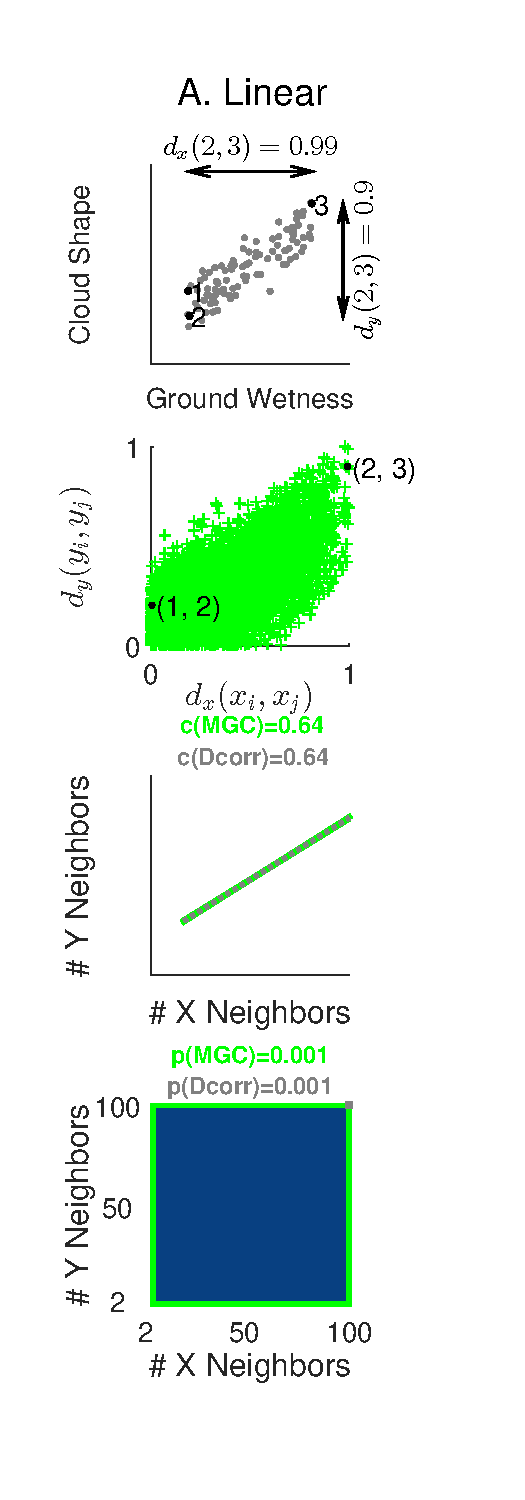
\includegraphics[width=1.0\textwidth]{../Figures/Fig1}
\caption{
Power of different methods on 20 different one-dimensional simulation settings, estimated by the empirical distributions of the test statistics under the null and the alternative on the basis of $10$,$000$ Monte-Carlo replicates.
Each panel shows empirical testing power on the absicca, and sample size on the ordinate.
MGC empirically achieves similar or better power than the previous state of the art approaches for nearly all sample sizes on most problems.}
\label{fig:1D}
\end{figure}

For the dimension $1$ scenario, we observe that MGC$\{$mcorr$\}$/$\{$dcorr$\}$/$\{$Mantel$\}$ either equals or is better than its corresponding global test. For dependencies that are close to linear (type 1-5), MGC usually yields similar testing powers as dcorr and mcorr, which are slightly better than HHG and Mantel; for the remaining nonlinear dependencies (type 6-19), HHG is the best among all global statistics, yet MGC is able to achieve similar or even better performance than HHG in most cases (the only exception is type 15, where HHG is still significantly better). 

Note that for all distributions other than the independent clouds, the empirical powers eventually increase to $1$ as the sample size increases, implying that all methods are consistent except the Mantel test, whose powers stay low in many nonlinear dependencies; and for the independent clouds, the empirical power of MGC is approximately at the type $1$ error level, so no false signal is detected. 

To better summarize the overall performance in the dimension $1$ simulations, we use the performance profiles \cite{DolanMore2002}, which provides an intuitive way for directly comparing a set of algorithms on a set of problems.  Briefly, each curve (profile) shows the relative performance of a given algorithm as a function of how far from the best algorithm it performed; therefore, higher curves and larger area under curve are better; a more detailed description is in appendix Section~\ref{appen:profiles}. For the dimension $1$ scenario, we fix the sample size by a power threshold, and draw the corresponding performance profiles of all methods in Figure~\ref{fig:pp}(a). To compare the performance profiles of each method with respect to different threshold choices, we also provide the area under curve of the performance profiles against the power threshold in Figure~\ref{fig:pp}(b).
\begin{figure}[htbp]
\subfloat[]{
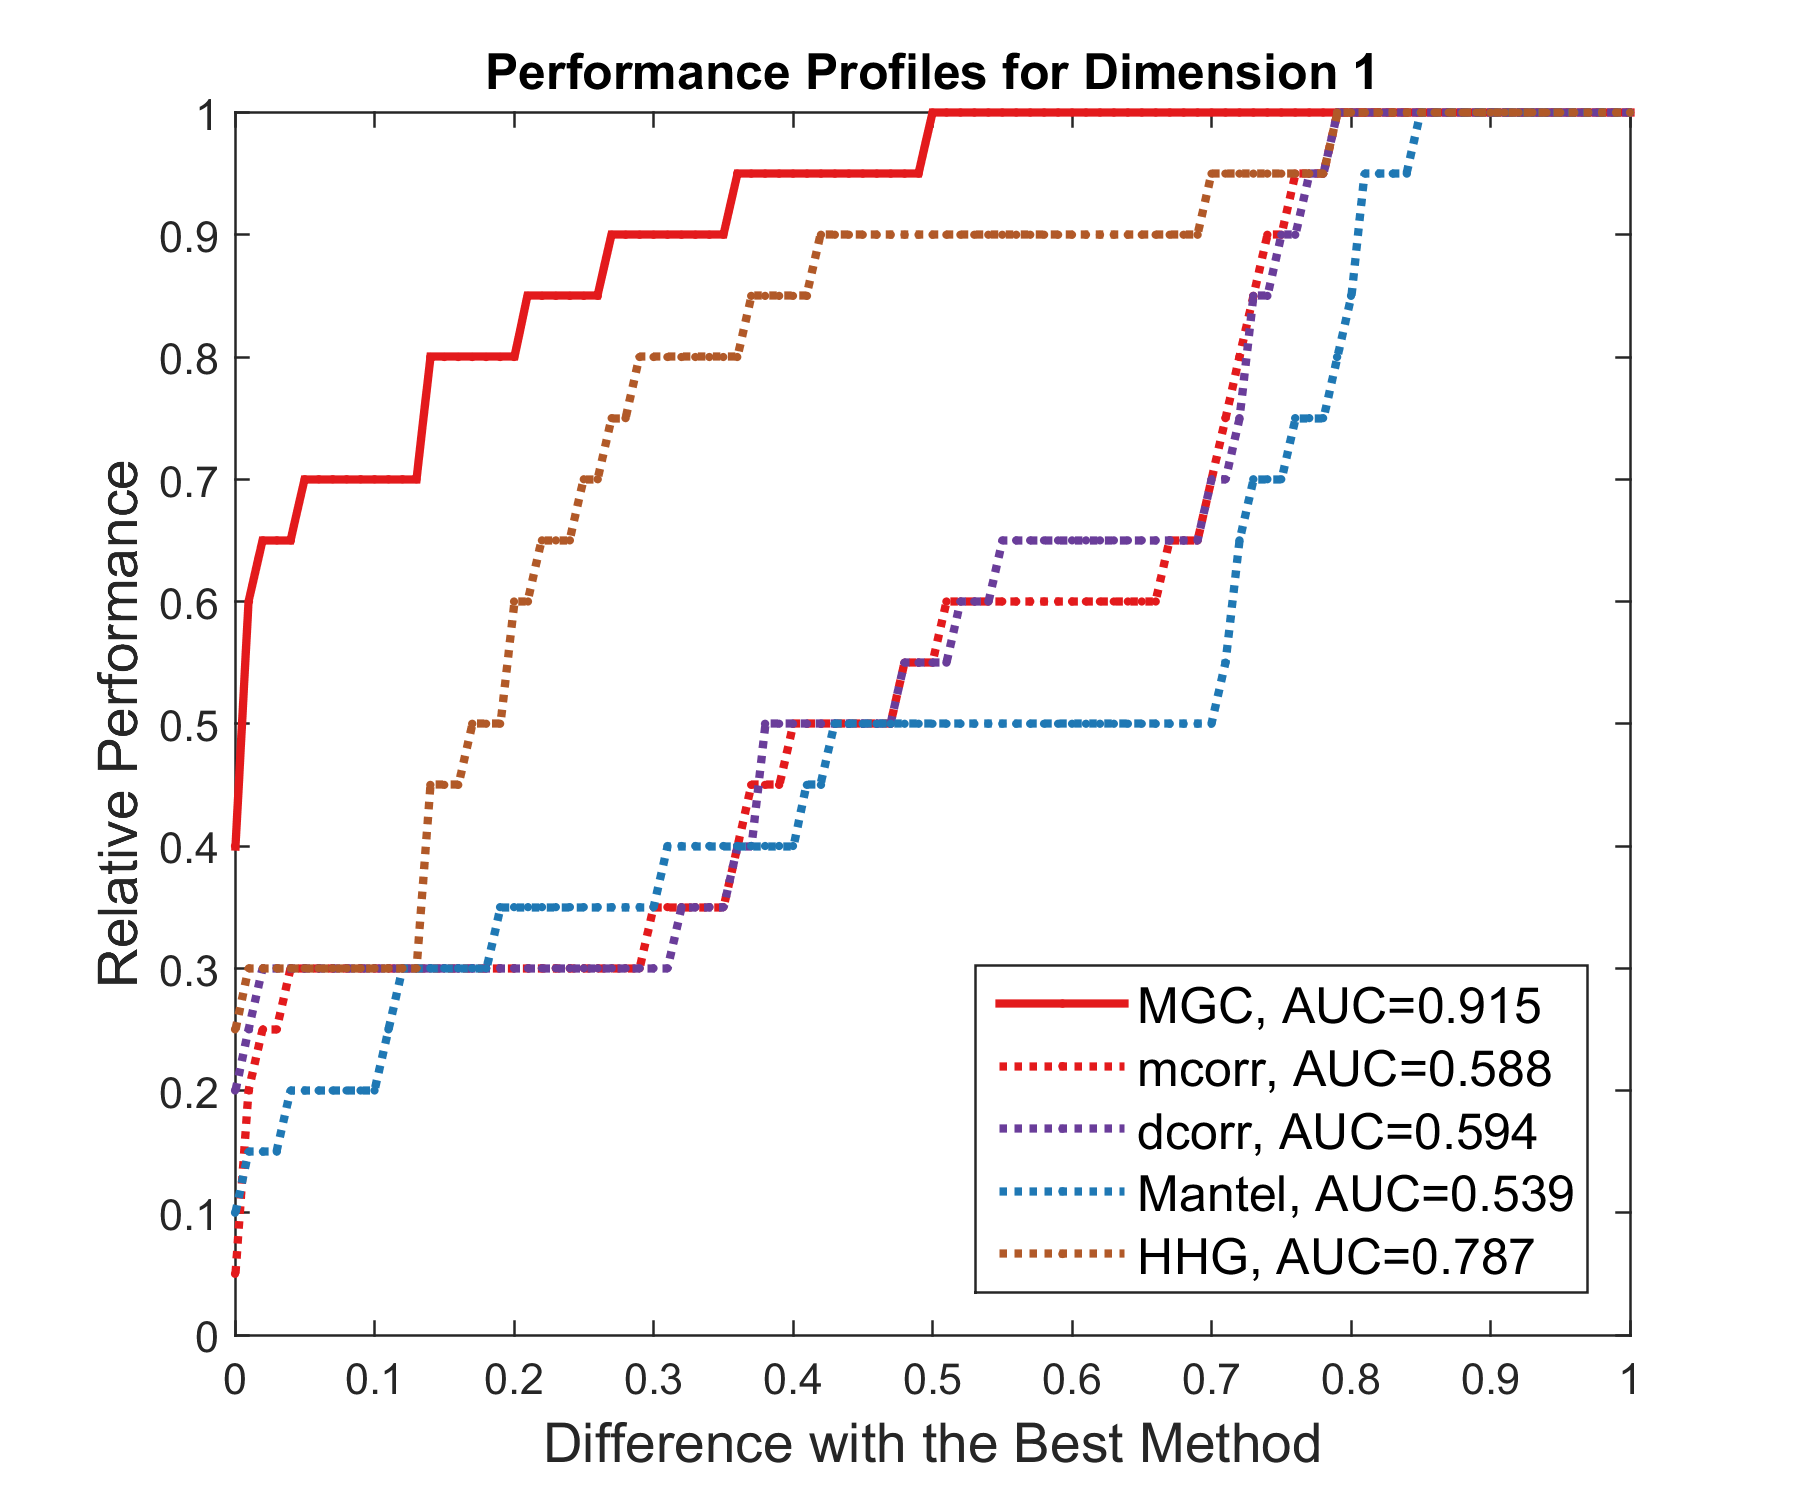
\includegraphics[width=0.5\textwidth]{../Figures/Fig3}
}
\hfil
\subfloat[]{
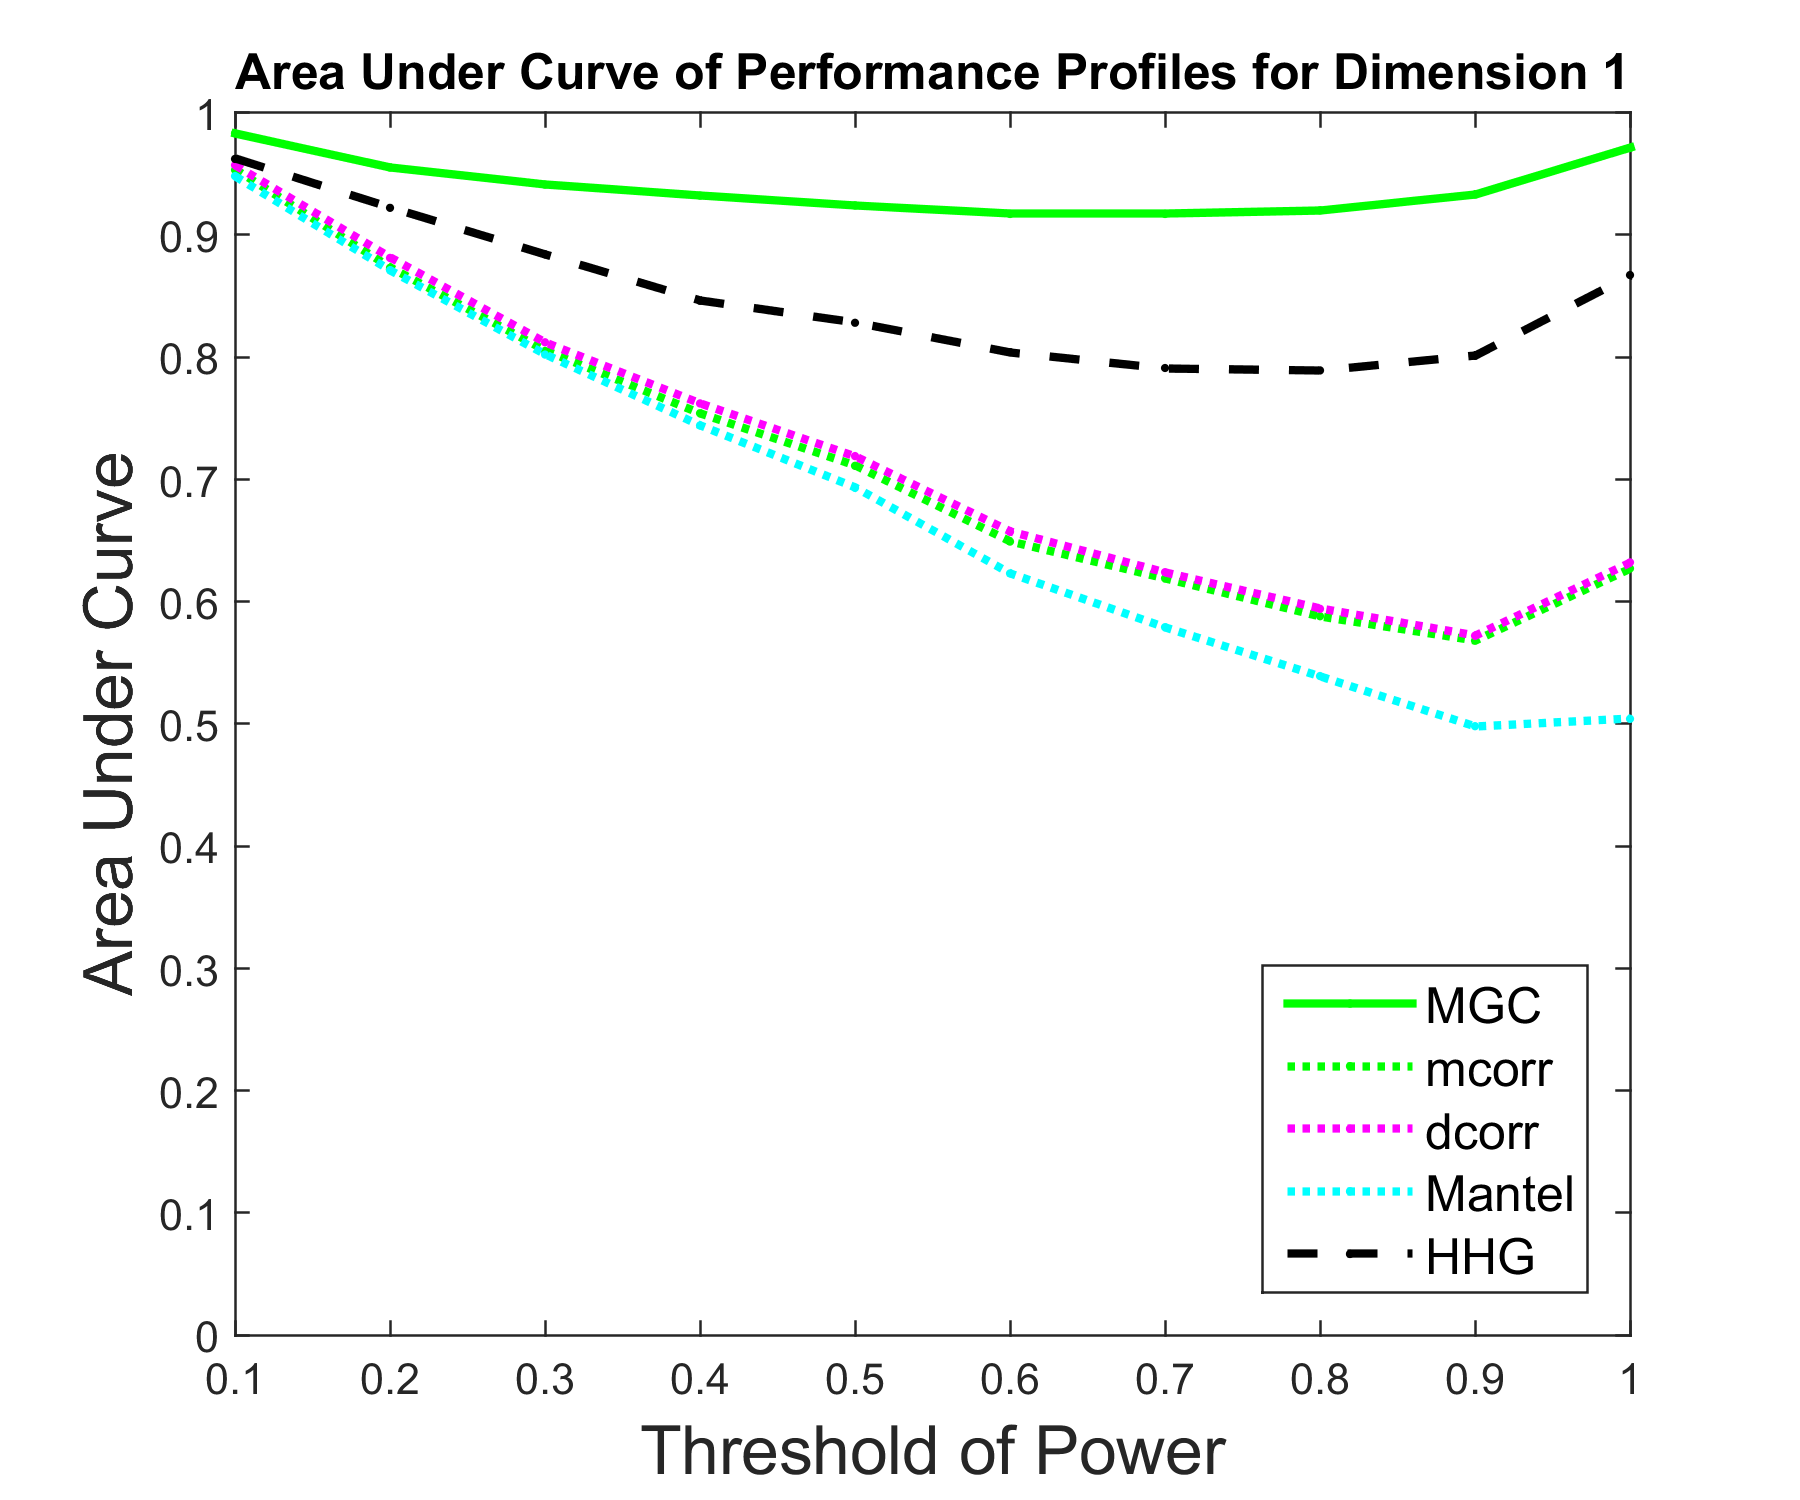
\includegraphics[width=0.5\textwidth]{../Figures/Fig4}
}
\hfil
\subfloat[]{
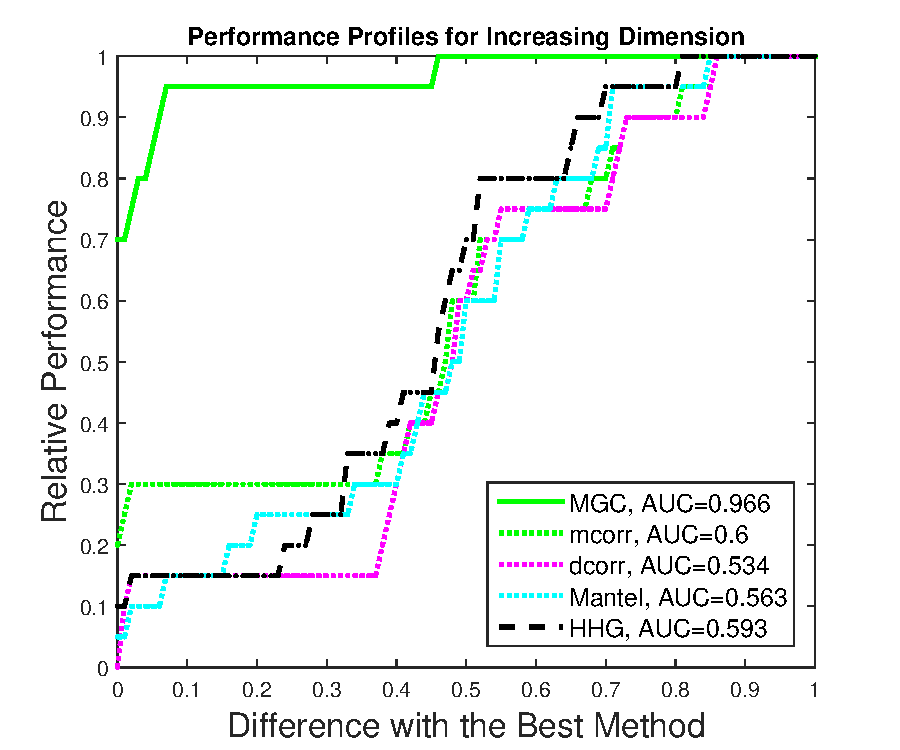
\includegraphics[width=0.5\textwidth]{../Figures/Fig7}
}
\hfil
\subfloat[]{
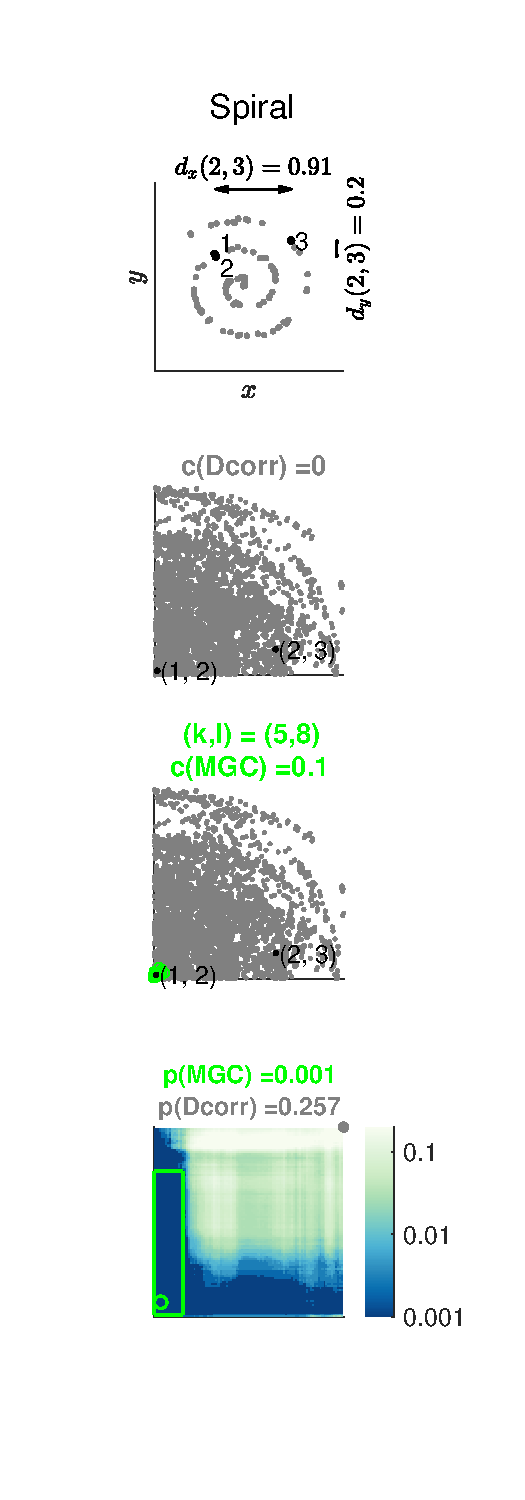
\includegraphics[width=0.5\textwidth]{../Figures/Fig8}
}
\caption{Quantitative comparisons of the power of the various algorithms across all simulations into a single number.  
(a) Performance profile plots comparing the different algorithms on all 1-dimensional problems at the first sample size $n$ of any testing power to exceed the power threshold 0.8. The legend provides the Area-Under-the-Curve (AUC) for each method; larger is better.
(b) AUC for each method sweeping over all different power thresholds, the higher the better.
(c) Same as (a) but for the high-dimensional simulations, at the last dimension of any testing power that is above the power threshold 0.5.
(d) Same as (b) but for the high-dimensional simulations.
It is clear that MGC outperforms the previous state of the art, regardless of function, sample size, and dimensionality.}
\label{fig:pp}
\end{figure}

We can clearly see from Figure~\ref{fig:pp}(a)(b) that MGC is indeed more reliable than all global tests in the dimension $1$ scenario. HHG is slightly better than dcorr/mcorr in the performance profiles, because there are more nonlinear simulations than linear in the $20$ dependencies, and HHG has a larger advantage for nonlinear dependency than its disadvantage in linear dependency; the global Mantel test has the lowest performance profile, but MGC$\{$Mantel$\}$ turns out to perform the best due to its advantage in type 11-13. 

%Note that the powers and performance profiles of MGC$\{$dcorr$\}$ and MGC$\{$Mantel$\}$ on the low dimensional simulations are provided in the appendix Section~\ref{appen:figure}, which perform slightly differently from MGC$\{$mcorr$\}$, but give the same interpretations regarding their advantages over all global statistics.


\subsection{High Dimensional Simulation Experiments}
\label{numer2}
In this subsection we consider the same $20$ distributions and the same testing procedures as in Section~\ref{numer1}, but under an increasing dimensional setting. For each dependency type, the testing powers are calculated against increasing $d_{x}$, with $d_{y}$ equals $d_{x}$ or $1$ depending on the particular distribution and the sample size fixed at $n=100$.

The empirical testing powers are again based on $r=10$,$000$ Monte-Carlo replicates at $\alpha=0.05$, and the optimal scale of MGC is estimated by $2$,$000$ MC replicates. The powers are shown in Figure~\ref{fig:nD} against $d_{x}$, and the performance profiles are provided in Figure~\ref{fig:pp}(c)(d): Figure~\ref{fig:pp}(c) draws the performance profiles of all methods at a fixed dimension determined by a power threshold; and Figure~\ref{fig:pp}(d) plots the area under curve of the performance profiles against the power threshold.

Like the dimension $1$ scenario, each MGC test either equals or is better than its corresponding global test in the increasing dimension scenario. In particular, for close to linear dependencies from type 1-5, MGC$\{$mcorr$\}$ and global mcorr are the best, whose powers deteriorate slower than the others; and for the remaining nonlinear dependencies (other than type 15), MGC has a significant advantage over the benchmarks due to its capability to better handle nonlinearity and high-dimensionality at the same time. The performance profiles of MGC in Figure~\ref{fig:pp}(c)(d) clearly reflect its superiority.

%Note that in one third of the high dimensional simulations (e.g. sine period, square, diamond), the testing powers quickly degrade to around $\alpha$ as the dimension increases for all methods, which imply that these complex dependencies at larger dimensions become too obscure to be detected at the limited sample size. Furthermore, the powers and performance profiles of MGC$\{$dcorr$\}$ and MGC $\{$Mantel$\}$ in the high dimensional simulations are also provided in the appendix Section~\ref{appen:figure}, which are no better than MGC$\{$mcorr$\}$ but still significantly surpass all global tests.


\begin{figure}[htbp]
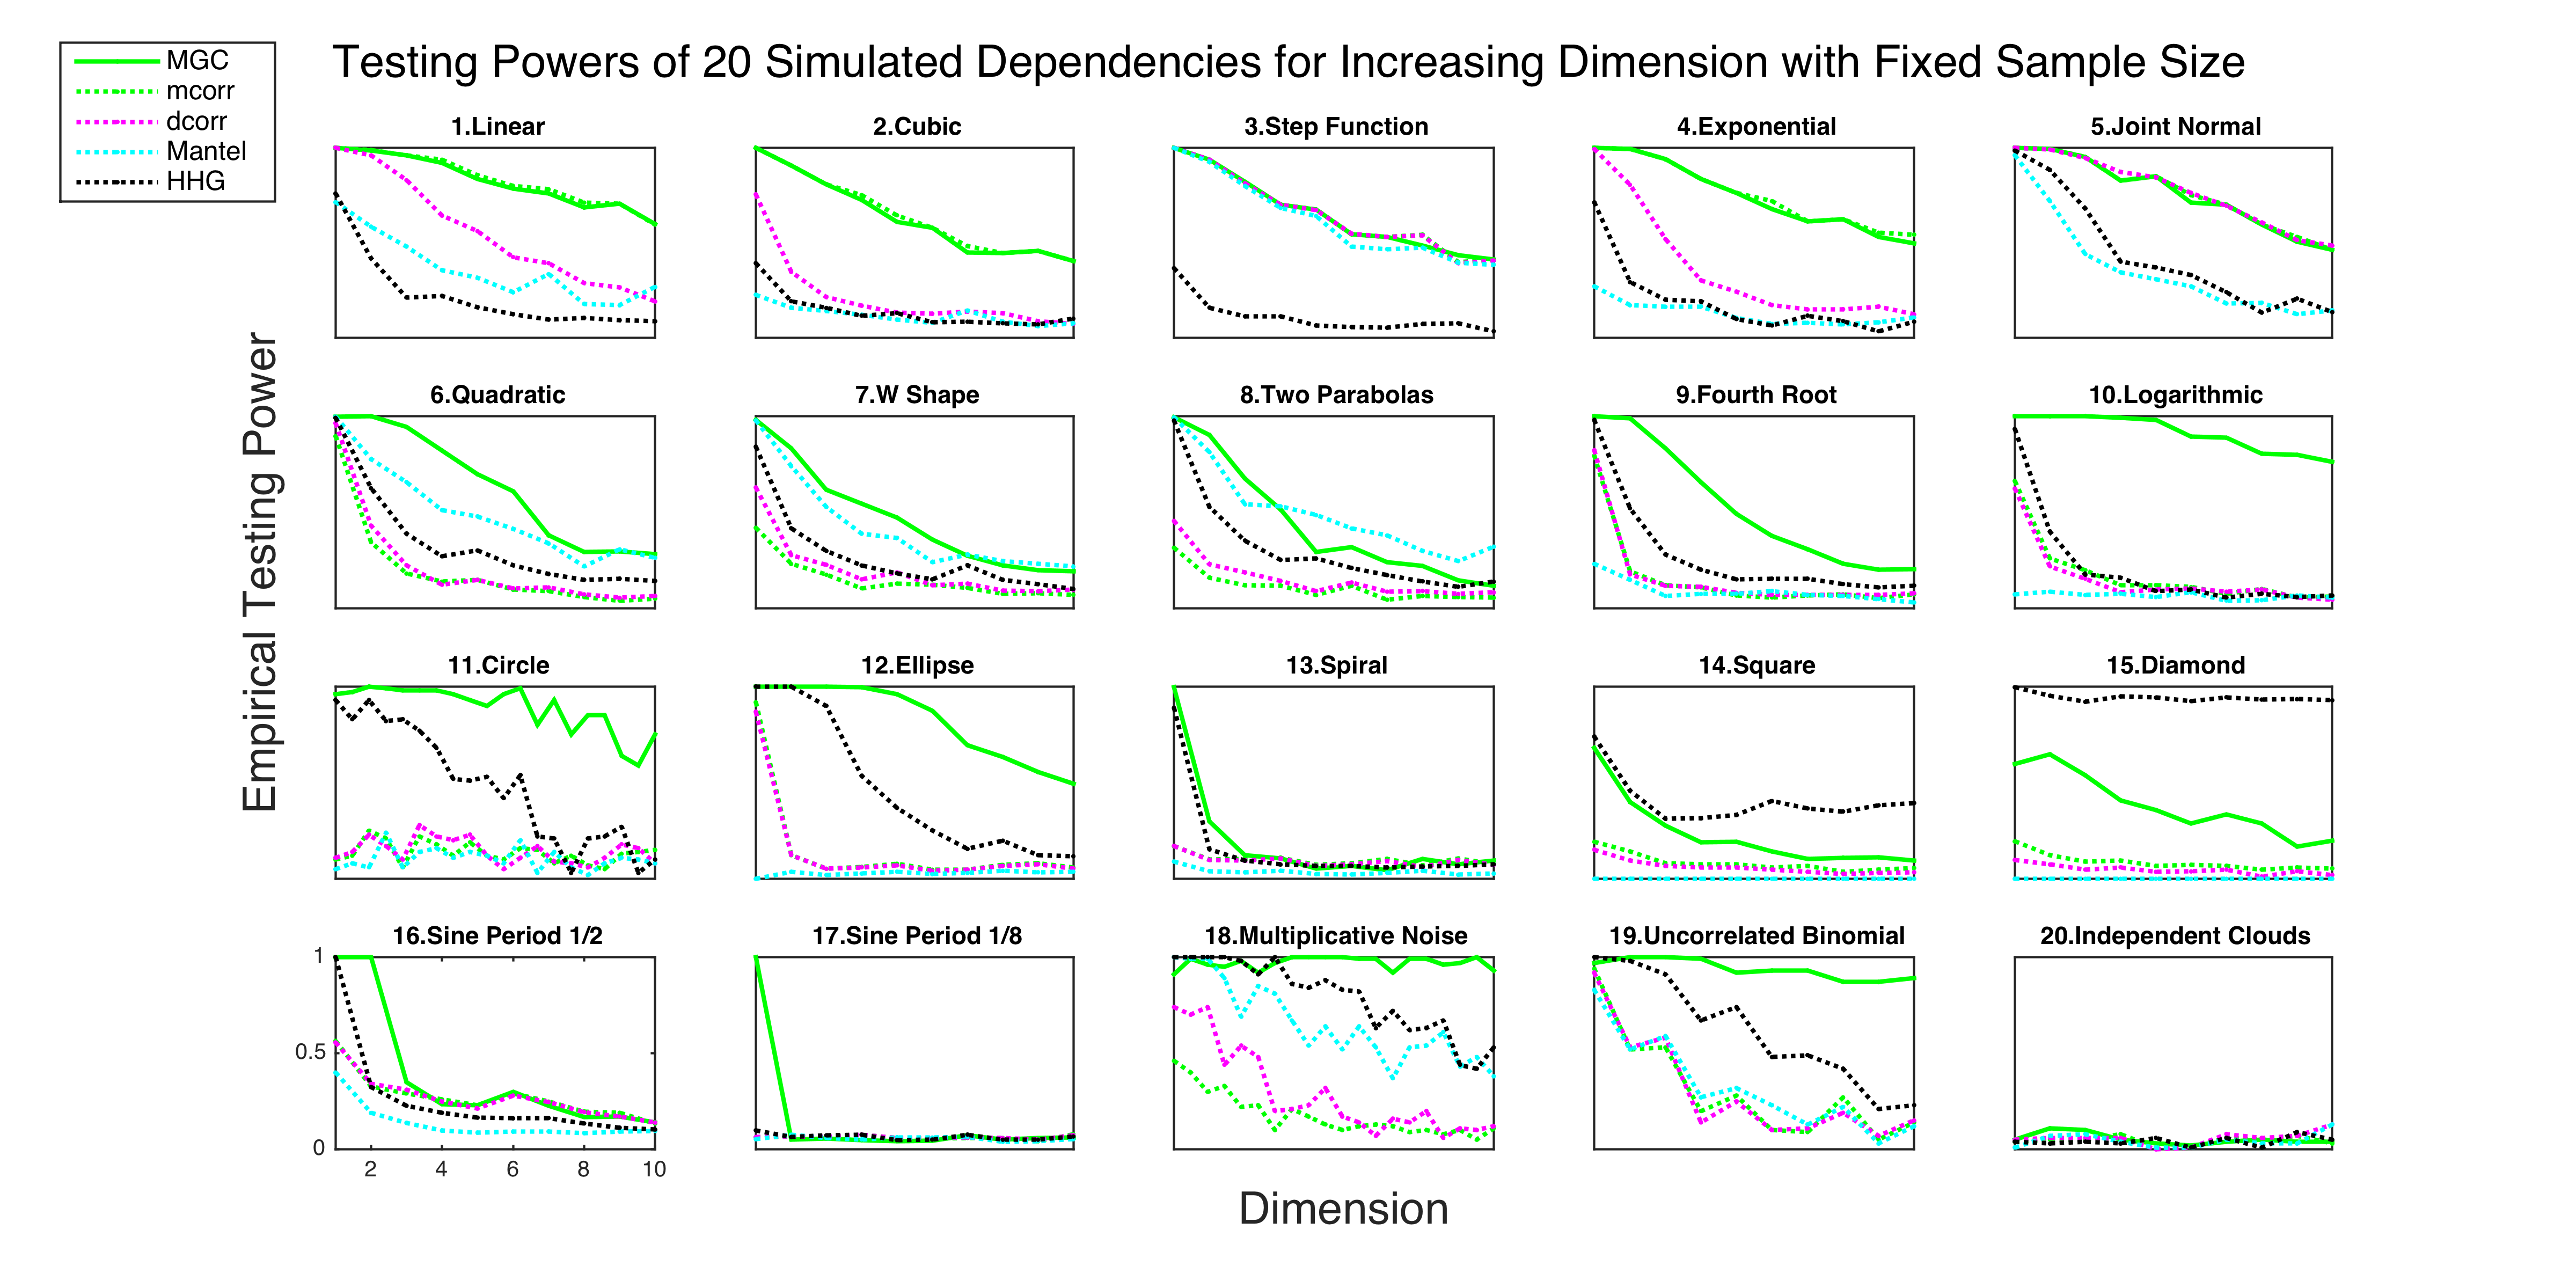
\includegraphics[width=1.0\textwidth]{../Figures/Fig5}
\caption{Power of different methods on 20 different simulation settings, for dimensionality ranging from 1 to 1000.  Details as in Figure~\ref{fig:1D}.
Again, our method empirically achieves as high or higher power than the previous state of the art approaches for nearly all sample sizes on nearly all problems and dimensions.
}
\label{fig:nD}
\end{figure}

\subsection{Discovery of Dependency Across Scales}
\label{main3}

In Figure~\ref{figSim2} we show how the powers of local statistics $\{g_{kl}\}$ change with respect to increasing neighborhood $k$ and $l$, for the low-dimension and high-dimension simulations. They are plotted at a fixed sample size and a fixed dimension by the same thresholds as the performance profiles figures in Figure~\ref{fig:pp}(a)(c). We can clearly see that for nearby neighborhoods, the powers of local tests can be very close, since the local statistics are strongly correlated with each other. %This implies that the optimal scale of MGC can be reasonably estimated by bootstrap; and even if the estimated scale is not the true optimal, it usually yields close to optimal testing power for MGC.

For dependencies that are close to linear (type 1-5), the best neighborhood choice is approximately at the largest scale, i.e., $k=l=n$. But for all other nonlinear dependencies (type 6-19), MGC almost always chooses a smaller scale, which is data dependent. For example, type 6 and type 7 are both polynomials of degree 2 with different coefficients, and the optimal scales of both are very similar to each other; type 9 and 10 have different functions but share similar dependencies from appendix Figure~\ref{fig0}, and their best scales are also close to each other; there also exists similar patterns between type 16 and 17.

\begin{figure}[htbp]
\subfloat[]{
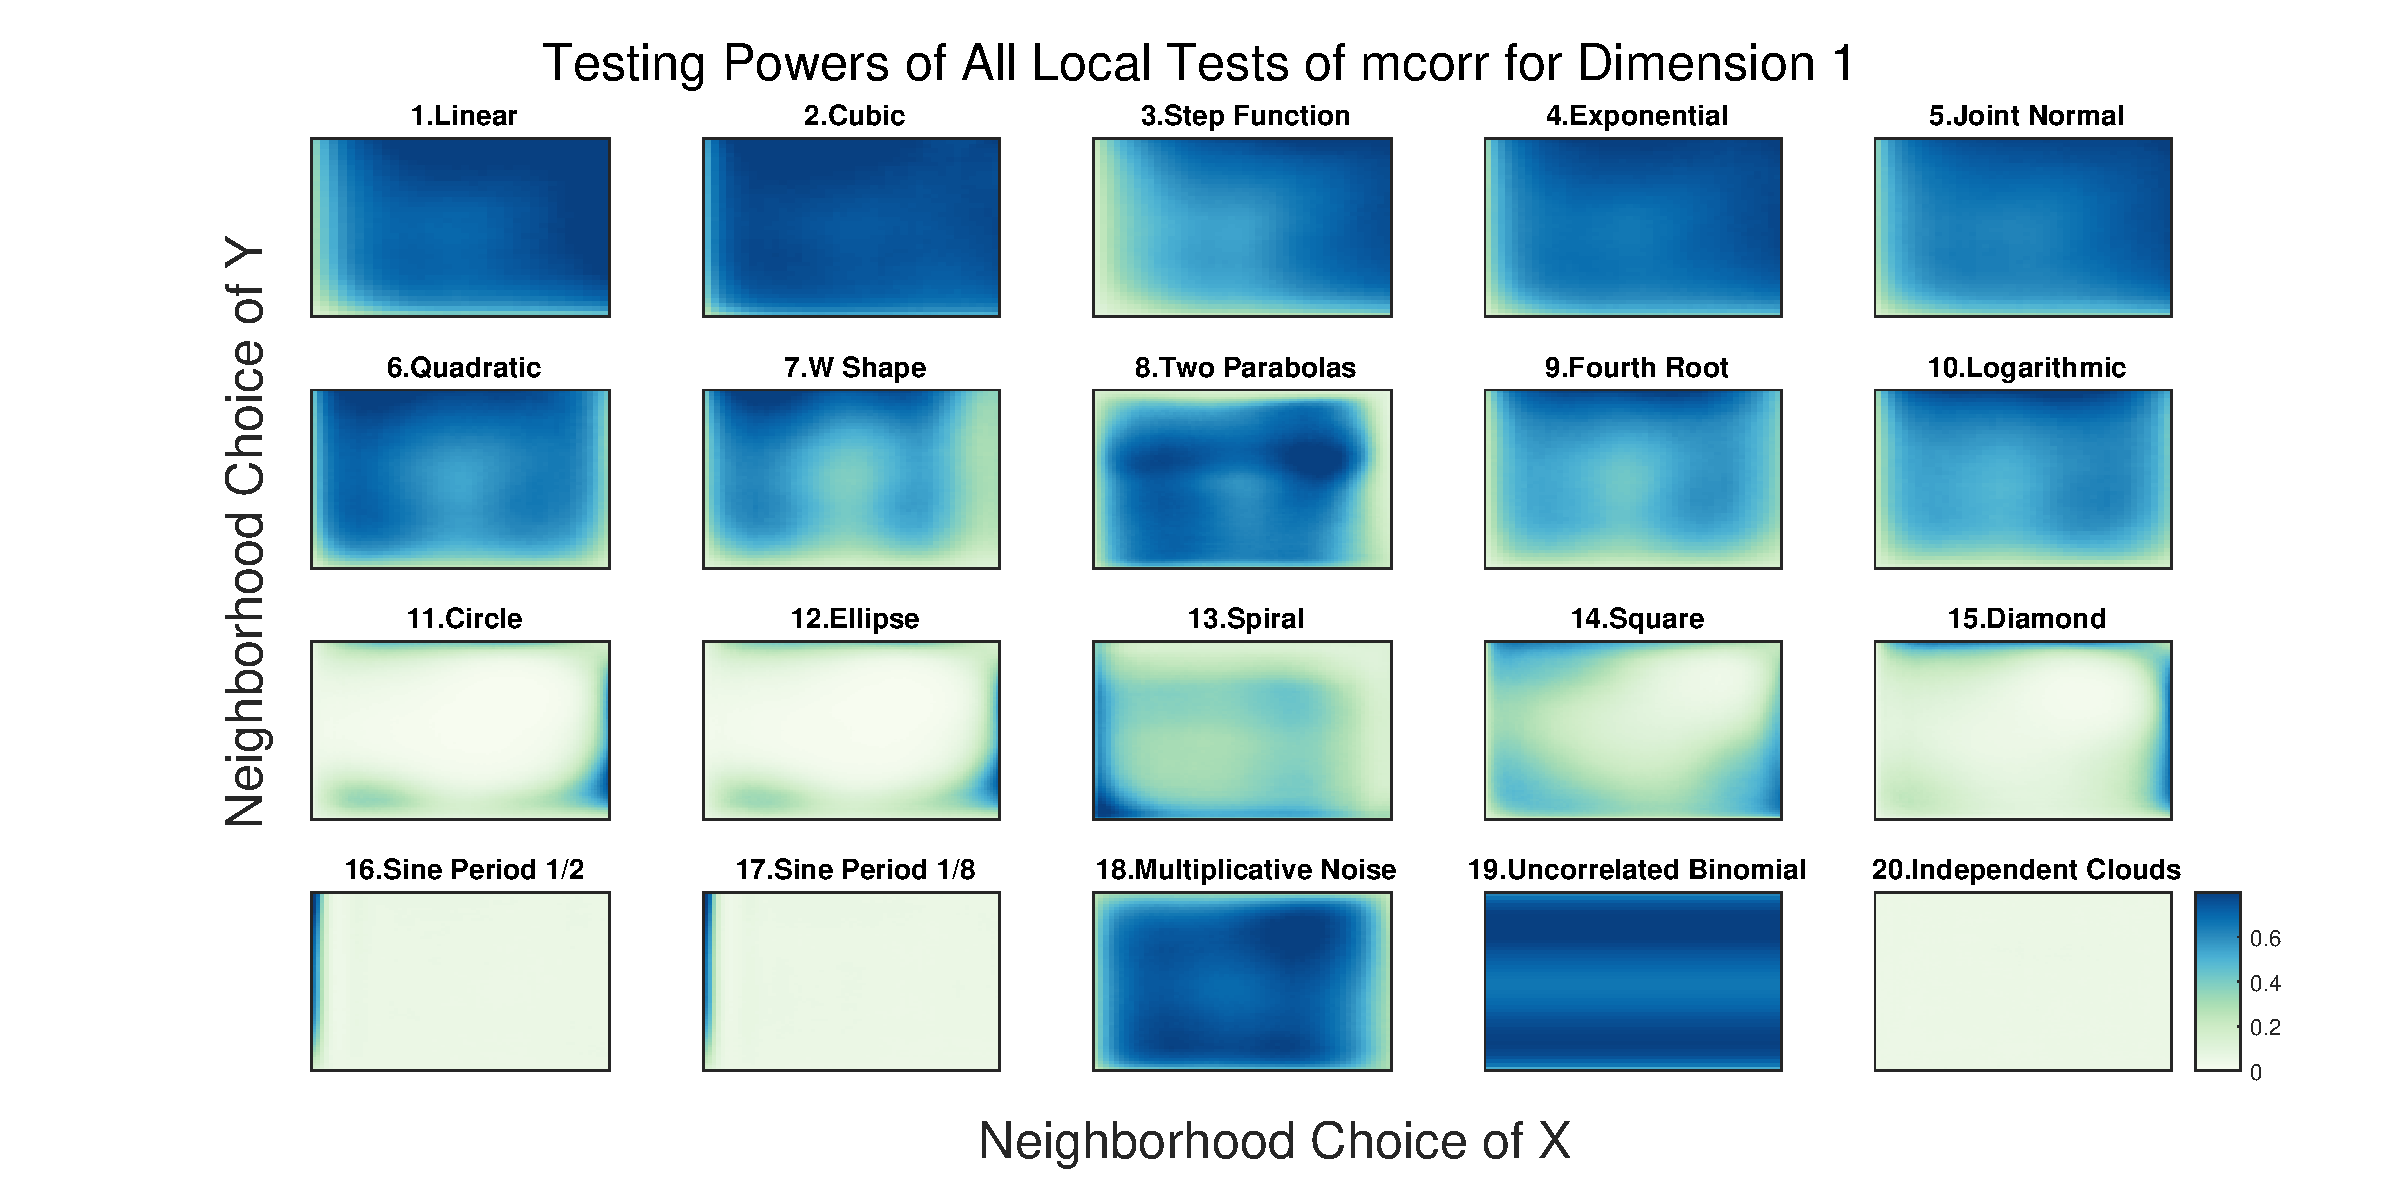
\includegraphics[width=1.0\textwidth]{../Figures/Fig2}
}
\hfil
\subfloat[]{
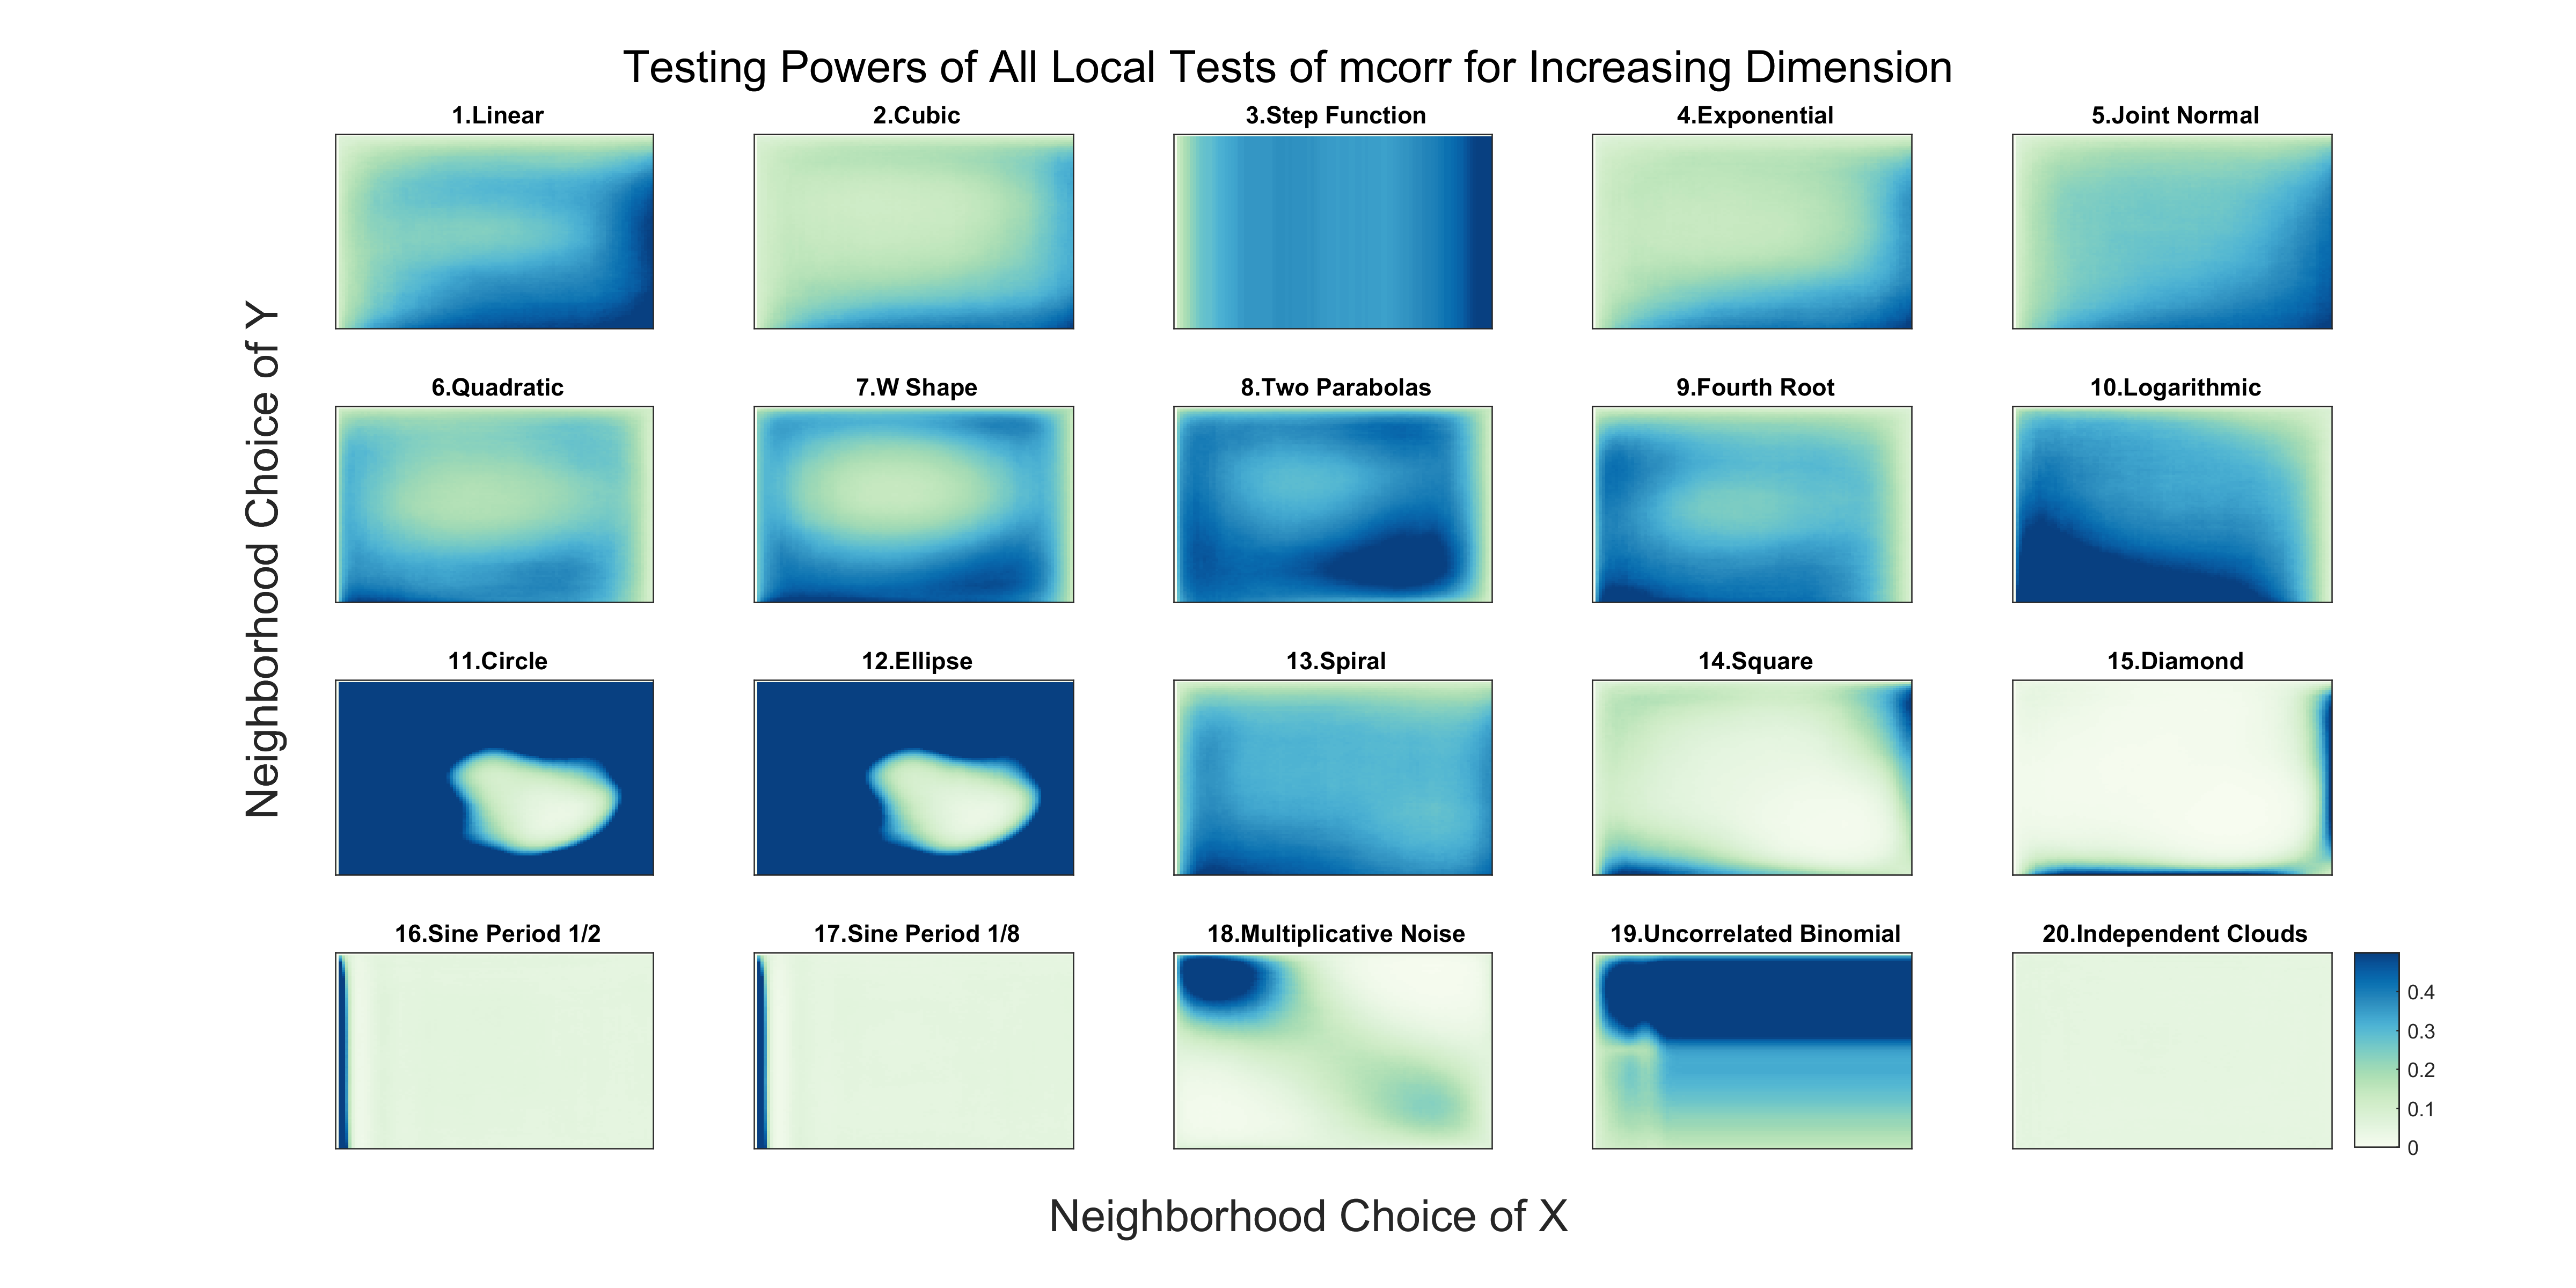
\includegraphics[width=1.0\textwidth]{../Figures/Fig6}
}
\caption{Testing Power Heat map of Local Statistics with respect to Neighborhood Choices for Dimension 1 and Increasing Dimension.
% Understanding how dependence varies with the local scale of the dependence.  
For each of the 20 panels, the abscissa denotes the number of neighbors for $X$, and the ordinate denotes the number of neighbors for $Y$.  Each different simulation yields a different surface, highlighting the importance of understanding local scale in terms of understanding the data.}
\label{figSim2}
\end{figure}

To characterize the above behaviors, in the following theorems we show that the testing power of MGC (by the permutation test) equals the testing power of the global test statistic under linear dependency, i.e., the optimal scale of MGC is at the largest. But under certain nonlinear dependency, the optimal scale is smaller such that MGC enjoys a better finite-sample testing power than the corresponding global statistic. 

\begin{thm}
\label{thm2}
Suppose $\mb{y}=c\mb{x}$ for a non-zero scalar $c$. Then for any $n$ and $\alpha$ it always holds that
\begin{equation}
\beta_{\alpha}(g) = \beta_{\alpha}(g_{nn}).
\end{equation}

Thus multiscale graph correlation is equivalent to the global correlation coefficient under linear dependency.
\end{thm}

\begin{thm}
\label{thm3}
There exists $f_{xy}$, $n$ and $\alpha$ such that 
\begin{equation}
\beta_{\alpha}(g) > \beta_{\alpha}(g_{nn}).
\end{equation}

Thus multiscale graph correlation can be better than its global correlation coefficient under certain nonlinear dependency.
\end{thm}
Note that Theorem~\ref{thm2} and Theorem~\ref{thm3} hold for MGC implemented by any of mcorr/dcorr/Mantel.

The proof of Theorem~\ref{thm3} is a constructive one, as it shows that local distances and local statistics outperform global ones even for the most modest nonlinear functions, such as a quadratic.  Because any function can be approximated by a polynomial expansion \cite{RudinBook}, the proof of Theorem~\ref{thm3} suggests that MGC is likely to outperform the corresponding global statistic on a wide variety of nonlinear functions, which is indeed the case throughout the numerical simulations.

\cs{Now I think the taylor expansion paragraph above is not right: any function can be approximated by polynomial expansion, does not imply the optimal scale is smaller than $n$.}
\jv{its not just that, its that even if you \emph{only} have to add a 2nd order term, already local beats global. }

\subsection{Real Data}
\label{numer3}
Here we apply MGC to test independence between brain features and personal characteristics from two different experiments, for which the data sets are relatively small in sample size due to the expensive data collection process. Based on the evaluation procedure in Section~\ref{appen:tests}, we report the p-value of each method from the permutation test, with the optimal scale of MGC estimated by repeated noisy samples of the given observations. Note that among the three MGC implementations, we only report the p-value of MGC$\{$mcorr$\}$ because MGC$\{$dcorr$\}$ and MGC$\{$Mantel$\}$ yield similar results.

The first experiment is to detect the relationship between the brain connectome and personality from \cite{AdelsteinEtAl2011}. The sample size is $n=42$, and each person has a $5$ dimensional personality data based on questionnaires and the five-factor personality model. Then the brain activity of each person is measured by fMRI for $197$ brain regions and $194$ time steps. Thus the brain connectome feature is high-dimensional while the personality data is low-dimensional. There seems to exist certain correlation between the brain activity and personality as experimentally shown in \cite{AdelsteinEtAl2011}, but whether the dependency can be detected from the raw data is the question here.

To apply our method, two distance measures are required for the two different data sources: for the personality data, the distance matrix is formed by the Euclidean distance directly; for the connectome data, we run a spectrum analysis for each region, bandpass and normalize it, then calculate the Kullback-Leibler divergence among regions and use the normalized Hellinger distance. Once the distance matrices are obtained, we apply the permutation test for $r=10$,$000$ random permutations, and show the p-values (the percentage that the test statistic between the permuted data is larger than the observed test statistic) of MGC, dcorr, mcorr, Mantel, and HHG in the first row of Table~\ref{table1}, with the smallest p-value highlighted in the table. 

In this experiment, only MGC yields significant p-value that is less than $0.05$, and the estimated optimal neighborhood choice is $k^{*}=9, l^{*}=4$ based on $2$,$000$ repeated noisy samples. No other method yields significant p-value, although HHG is quite close. We also show the p-value heat map of all local tests with respect to different choices of neighborhoods in Figure~\ref{figReal}(a), and we can clearly see a local structure in the data that yield significant p-values for adjacent scales.

\cs{we should replace the above experiment by others, or just abandon it; since the MGC p-value is now 0.15 for connectome vs personality, after the current bias adjustment, which is higher than HHG; and no method yields significance for this data set now.}
%Note that if we use MGC by dcorr rather than mcorr, the p-value is no longer significant: this implies a high-dimensional structure in the dependency, which is indeed the case for the connectome data. 

%Note that the distance measure (especially for the connectome data) may not be the most appropriate for detecting dependency, and it is possible that HHG and dcorr may yield better p-values under different metrics.

\begin{table*}[!t]
\footnotesize
\renewcommand{\arraystretch}{0.5}
\centering
{\begin{tabular}{|c||c|c|c|c|c|c|c|}
\hline
Testing Method & MGC & mcorr & dcorr & Mantel & HHG \\
\hline
Connectome x Personality & $\textbf{0.2723}$ & $0.3203$ & $0.6606$ & $0.9869$  & $0.0583$ \\
\hline
Left Brain vs Disorder  & $\textbf{0.0192}$ & $0.0880$ & $0.0784$ & $0.0387$ & $0.0371$ \\
\hline
Right Brain vs Disorder & $\textbf{0.0084}$ & $0.1197$ & $0.1123$  & $0.0812$ & $0.0878$\\
\hline
Voxel vs non-existent Stimulus & $0.0570$ & $0.0503$ & $0.0495$  & $0.0671$ & $0.0312$\\
\hline
\end{tabular}
\caption{The Empirical P-Values in the Permutation Test}
\label{table1}
}
\end{table*}

\begin{figure}[htbp]
\centering
\subfloat[]{
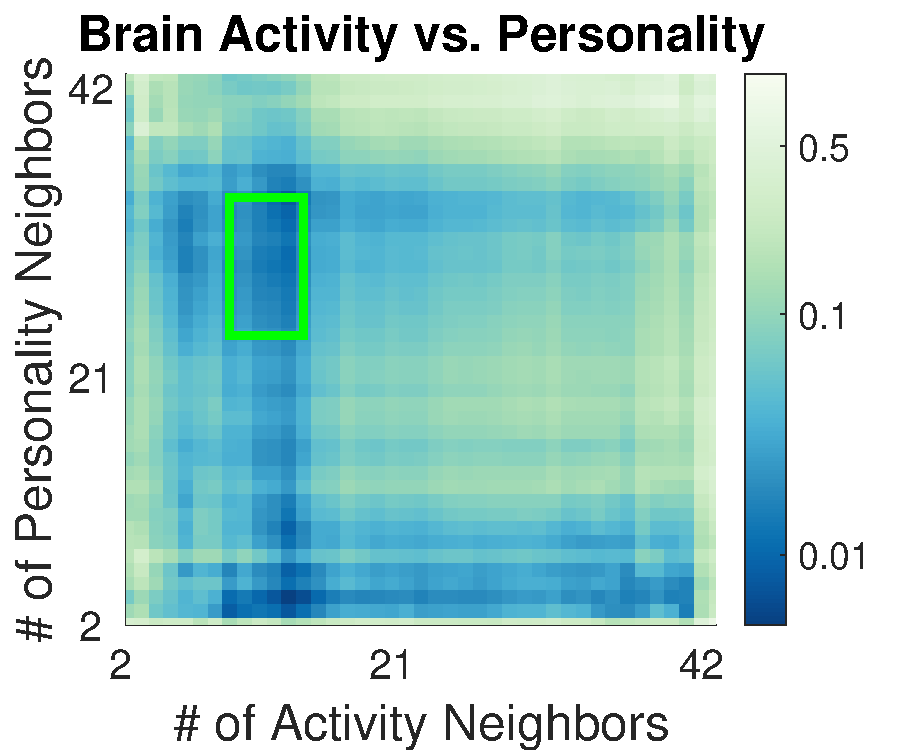
\includegraphics[width=0.48\textwidth]{../Figures/FigReal1}
}
\hfil
\centering
\subfloat[]{
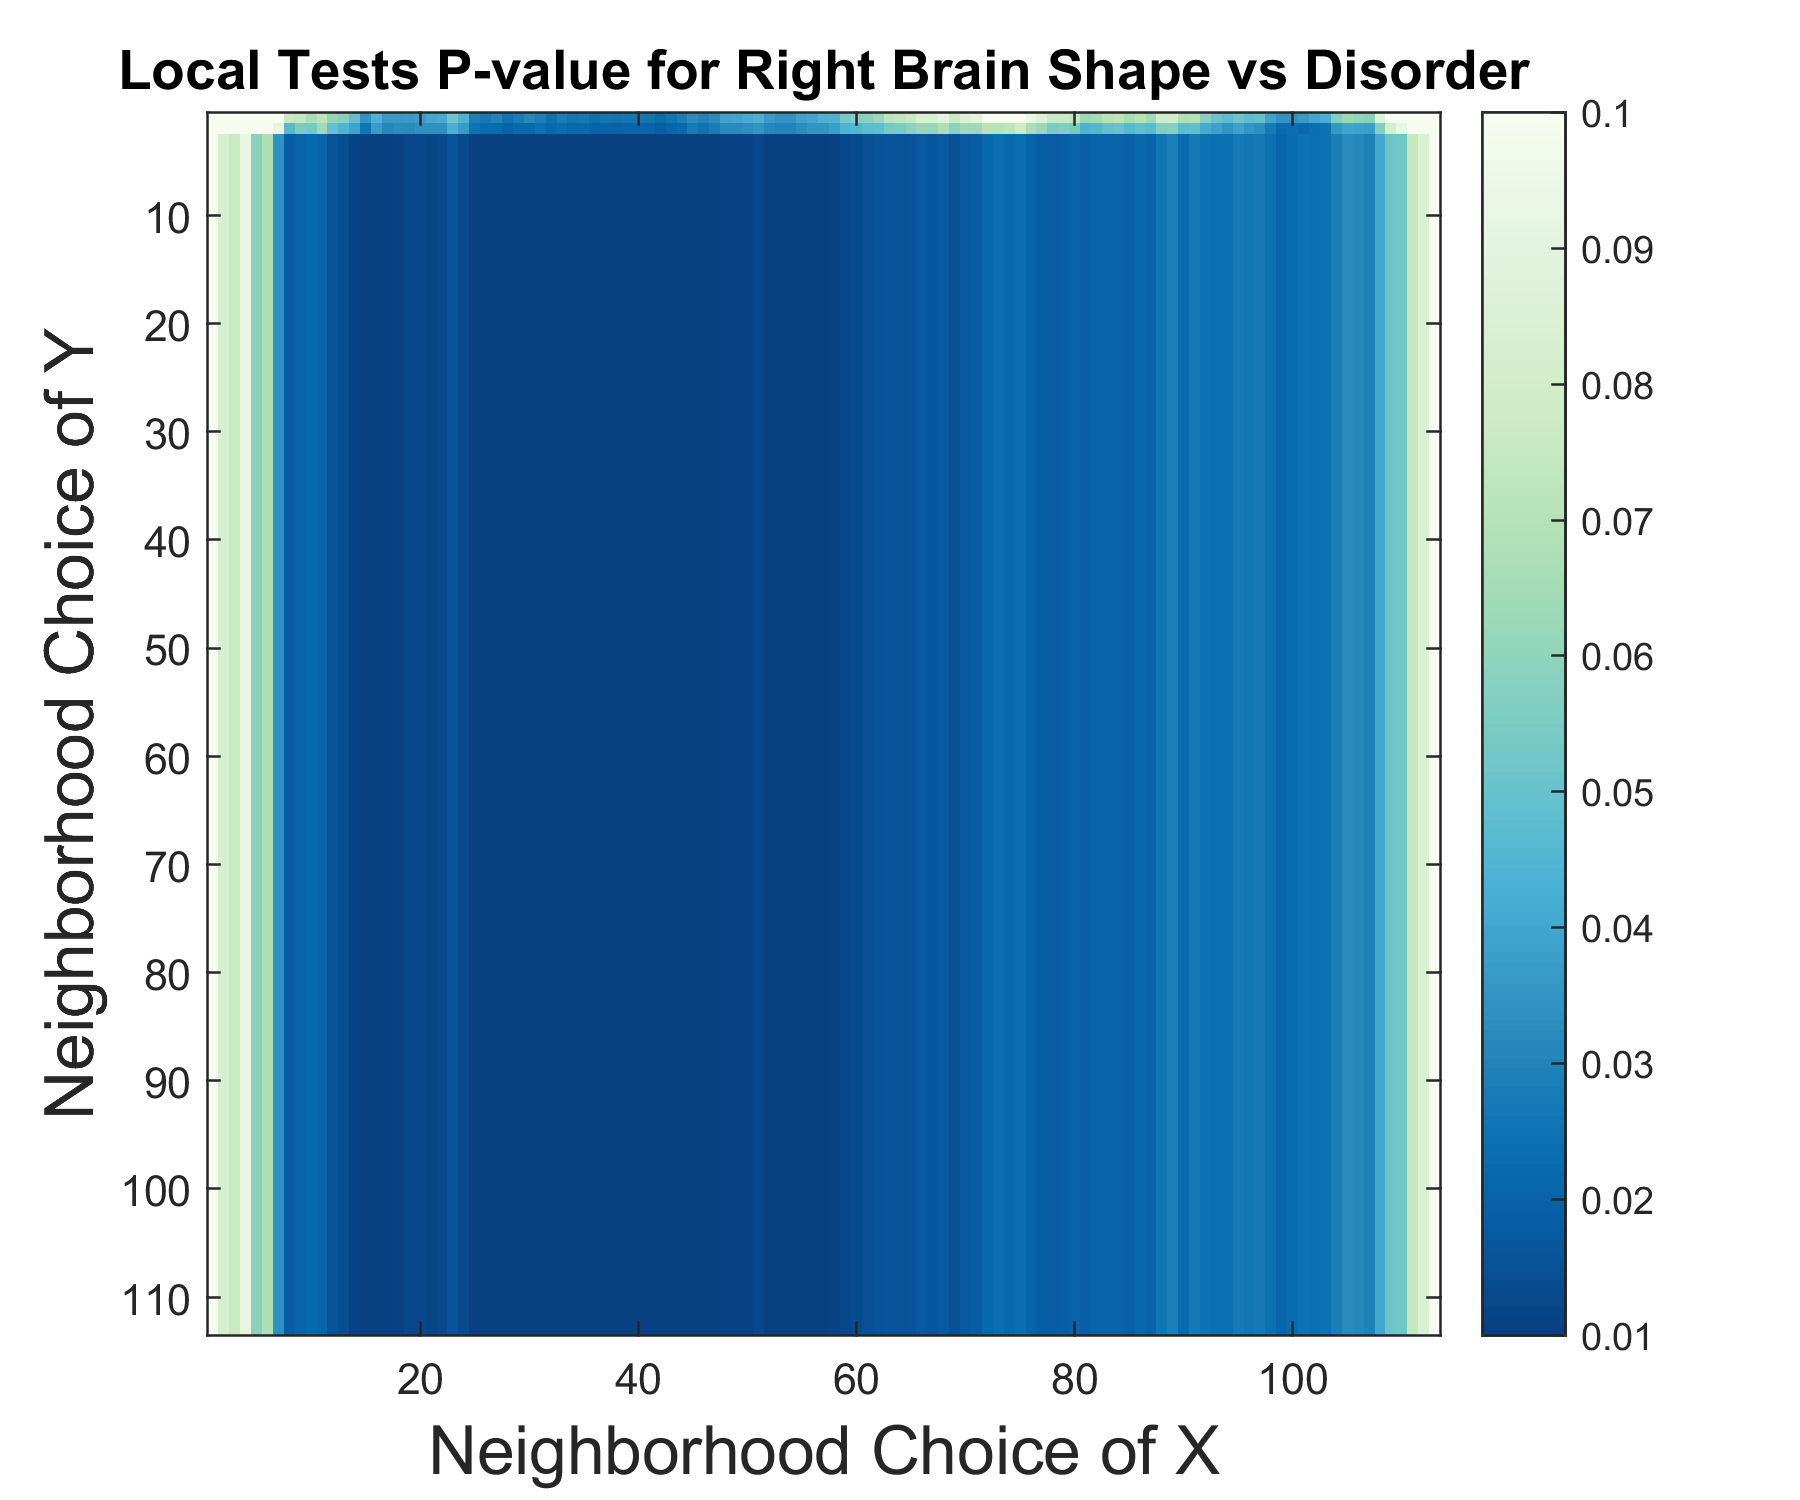
\includegraphics[width=0.48\textwidth]{../Figures/FigReal2}
}
\hfil
\centering
\subfloat[]{
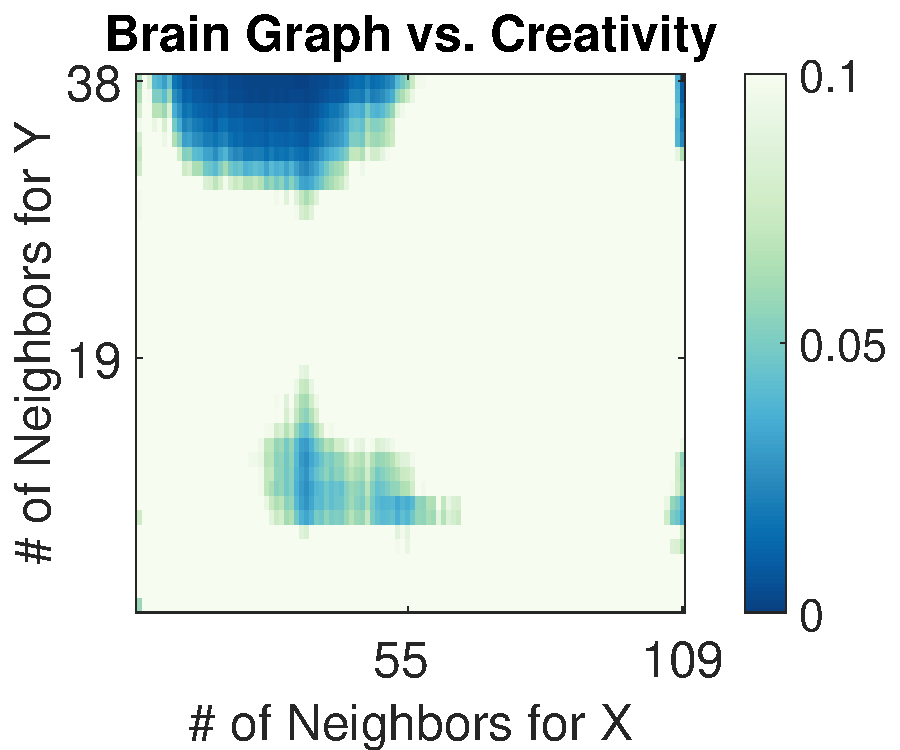
\includegraphics[width=0.48\textwidth]{../Figures/FigReal3}
}
\caption{P-Value Heat map of Local Tests with respect to Different Neighborhood Choice.  In the real data, for the Connectome vs. personality, global structure is inadequate to reveal any dependence between the two modalities.  For the brain shape vs. disorder status,  global distances are close to adequate, and most neighborhoods yield significant p-values.}
\label{figReal}
\end{figure}

Next we carry out the same testing procedure on another experiment regarding brain hippocampus shape and major depressive disorder. There are $n=114$ subjects, and the brain images of each person are obtained by high resolution MRI scans on the hippocampus; and we also have available a categorical vector containing the disorder information, including clinically depressed subject, high-risk subject, and non-affected subject. There has been evidences that relate major depressive disorder to the hippocampus shape in \cite{ParkEtAl2011} and \cite{PosenerEtAl2003}, and we would like to test the significance of such relationship in the data. 

The brain data is transformed into two dissimilarity matrices representing the left and right hippocampus data based on landmark matching (see \cite{ParkEtAl2011} for more details on data processing). The disorder information vector is transformed into its Euclidean distance with all off-diagonal entries added by $1$, so that only the diagonals are zero, and subjects of the same disorder status have smaller distance than subjects of different disorder status. 

We consider two hypothesis tests: testing dependency between the left brain and major depressive disorder, and testing dependency between the right brain and major depressive disorder. The resulting p-values are reported in the second and third rows of Table~\ref{table1}. For testing between the left brain and the disorder, MGC/HHG/Mantel yield significant p-values with dcorr/mcorr being slightly higher than significance; for testing between the right brain and the disorder, only MGC yields significant p-value, with all global tests higher than significance. Note that if we use MGC$\{$dcorr$\}$ or MGC$\{$Mantel$\}$, they also yield significant p-values similar to MGC$\{$mcorr$\}$.

The p-value heat maps of all local tests are provided in Figure~\ref{figReal}(b)(c), where we observe that there exist many scales that are close to optimal; and the estimated largest optimal scales are $k^{*}=44,l^{*}=114$ and $k^{*}=37,l^{*}=114$ respectively. Note that the p-values of local test statistics at a given $k$ are the same throughout any $l \in [3,114]$, because we use minimum rank for ties and the largest rank is $2$ for the disorder distance matrix; and if we test dependency between the left and right brain, all p-values become $0$, indicating a strong linear dependency between the left and right brain.

% Furthermore, if we assume that the left brain shape and the right brain shape have the same underlying distribution, we may pick a consistent optimal scale by maximizing the sum of local testing powers. In this case the optimal scale becomes $k^{*}=37, l^{*}=114$, and the MGC p-values become $0.0224$ and $0.0092$ respectively, which are in fact lower than the MGC p-values in Table~\ref{table1} using separate optimal scales.

% and if we assume that the left brain data distributes the same as the right brain data such that one optimal scale should be used for both testing tasks, then either $(23,114)$ or $(20,114)$ can yield significant p-values as observed from Figure~\ref{figReal}(b)(c).

%We can observe from the heat map of MGC that there is a clear threshold in the local structure most neighborhood choices after certain threshold yields significant p-values, and MGC with mcorr performs similarly as MGC with dcorr. They imply that the dependency between the brain data and the disease data is probably cross-region, close to linear and low-dimensional. Furthermore, the left brain seems to be more correlated with the disease than the right brain, as testing between $LML$ and $D$ yields smaller p-values than testing between $LMR$ and $D$.

The last experiment uses MGC to test independence between brain voxel activities and non-existent stimulus, similar to the experiment in \cite{EklundKnutsson2012}; and we take the BNU1 data for illustration. Two fMRI scans are done for a total of $50$ persons, including $200$ regions of interest for $200$ time steps; then we generate an independent stimulus by a standard normal distribution with respect to the time scales, i.e., the stimulus is the same for all brain regions and all persons at a given time steps.

We use the first scan for testing. For each region, we can form a $200 \times 200$ distance matrices by the Euclidean distance with respect to the time steps; and we can form another distance matrix for the stimulus, and test independence between each region and the stimulus for significance. By using $10000$ permutations to yield the p-value, each voxel is declared significant when the p-value is less than $\alpha=0.05$. 

Since the stimulus is independent, the testing power, i.e., the percentage of brain regions declared significant, should be close to $\alpha$. Indeed, all methods including MGC return power no larger than $0.07$ as shown in Table~\ref{table1}.

\section{Discussion}
\label{conclu}

\paragraph{Summary}

In short, we propose multiscale graph correlation to test independence between data sets, which has been shown to be perform well for testing independence on data of small sample size, high-dimensionality, linearity or nonlinearity. It not only enjoys theoretical guarantee such as being consistent in testing independence, but also exhibits superior numerical performances in a comprehensive simulation setting and real data experiments, comparing to other popular methods.


\paragraph{Next Steps}

one-sample, two-sample test by the local variants, group testing, anova, regressing out other covariates (local partial correlation), screening, metric spaces.

different test statistics: there are many possible ways to generate the null distribution, including permutation, but also t-test (as in the mcorr paper \cite{SzekelyRizzo2013a} and the asymptotic distribution derived from \cite{GrettonEtAl2012}), wilcoxon signed rank test, etc..

scaling up via FlashX?

\section*{Acknowledgment}
\addcontentsline{toc}{section}{Acknowledgment}
This work was partially supported by 
% 
National Security Science and Engineering Faculty Fellowship (NSSEFF), 
% 
Johns Hopkins University Human Language Technology Center of Excellence (JHU HLT COE), 
% 
Defense Advanced Research Projects Agency's (DARPA) SIMPLEX program through SPAWAR contract N66001-15-C-4041, 
% 
and the XDATA program of the Defense Advanced Research Projects Agency (DARPA) administered through Air Force Research Laboratory contract FA8750-12-2-0303.



\appendix
\setcounter{figure}{0}
\renewcommand\thefigure{\arabic{figure}} 

\section{Functions}
\label{appen:function}

Here we list the distributions of the $20$ dependencies used in the simulation sections, which are based on a combination of the numerical simulations in \cite{SzekelyRizzoBakirov2007, SimonTibshirani2012, SimonTibshirani2012, GorfineHellerHeller2012} with some adjustments (such as the inclusion of additional noise and an extra weight vector) to better compare all methods in our low and high dimension scenarios.

For the purpose of the increasing dimension scenario, we denote $\mb{x}_{d}$ as the $d$th dimension of $\mb{x}$, and denote $w$ as a size $d_{x} \times 1$ vector with $w_{d}=\frac{1}{d}$. So $w\T \mb{x}$ is a dimension $1$ random variable that is a decaying weighted summation of $\mb{x}=[\mb{x}_{1};\ldots;\mb{x}_{d_{x}}]$; and $w\T \mb{x}$ equals $\mb{x}$ when $d_{x}=1$. In the following, $\mb{u}, \mb{v}$ are auxiliary random variables, $\mc{U}$ denotes the uniform distribution, $\mc{B}$ denotes the Bernoulli distribution, $\mc{N}$ denotes the normal distribution, $c$ is a scalar constant to control the noise level, and $\mb{\epsilon}$ denotes the standard normal distribution for white noise unless mentioned otherwise. The resulting pair of random variables $(\mb{x},\mb{y})$ are used to generate sample data for testing dependency.

\setcounter{equation}{0}
\begin{compactenum}
\item Linear: $\mb{x} \sim \mc{U}(-1,1)^{d_{x}}$, 
\begin{align*}
\mb{y} &=w\T \mb{x}+c\mb{\epsilon}.
\end{align*}
\item Cubic: $\mb{x} \sim \mc{U}(-1,1)^{d_{x}}$, 
\begin{align*}
\mb{y} &=128(w\T \mb{x}-\frac{1}{3})^3+48(w\T \mb{x}-\frac{1}{3})^2-12(w\T \mb{x}-\frac{1}{3})+80c\mb{\epsilon}.
\end{align*}
\item Step Function: $\mb{x} \sim \mc{U}(-1,1)^{d_{x}}$, 
\begin{align*}
\mb{y} &=\mb{I}(w\T \mb{x}>\hat{E}(w\T \mb{x}))+c\mb{\epsilon},
\end{align*}
where $\hat{E}(w\T \mb{x})$ denotes the sample mean of $w\T \mb{x}$ and $\mb{I}$ is the indicator function. 
\item Exponential: $\mb{x} \sim \mc{U}(0,3)^{d_{x}}$, 
\begin{align*}
\mb{y} &=exp(w\T \mb{x})+10c\mb{\epsilon}.
\end{align*}
\item Joint normal: Let $\rho=\frac{1}{2d_{x}}$, $I_{d_{x}}$ as the identity matrix of size $d_{x} \times d_{x}$, $J_{d_{x}}$ as the matrix of ones of size $d_{x} \times d_{x}$, and $\Sigma = \begin{bmatrix} I_{d_{x}}&\rho J_{d_{x}}\\ \rho J_{d_{x}}&I_{d_{x}} \end{bmatrix}$. Then let $(\mb{x},\mb{u}) \sim \mc{N}(0, \Sigma)$, $\mb{\epsilon} \sim \mc{N}(0, I_{d_{x}})$,and $$\mb{y}=\mb{u}+0.5c\mb{\epsilon}.$$ 
\item Quadratic: $\mb{x} \sim \mc{U}(-1,1)^{d_{x}}$,
\begin{align*}
\mb{y}&=(w\T \mb{x})^2+0.5c\mb{\epsilon}.
\end{align*}
\item W Shape: $\mb{x} \sim \mc{U}(-1,1)^{d_{x}}$, $\mb{u} \sim \mc{U}(-1,1)^{d_{x}}$,
\begin{align*}
\mb{y}&=4( ( (w\T \mb{x})^2 - \frac{1}{2} )^2 + w\T \mb{u}/500 )+0.5c\mb{\epsilon}.
\end{align*}
\item Two Parabolas: $\mb{x} \sim \mc{U}(-1,1)^{d_{x}}$, $\mb{\epsilon} \sim \mc{U}(0,1)$, $\mb{u} \sim \mc{B}(0.5)$,
\begin{align*}
\mb{y}&=( (w\T \mb{x})^2  + 2c\mb{\epsilon}) \cdot (\mb{u}-\frac{1}{2}).
\end{align*}
\item Fourth Root: $\mb{x} \sim \mc{U}(-1,1)^{d_{x}}$,
\begin{align*}
\mb{y}&=|w\T \mb{x}|^\frac{1}{4}+\frac{c}{4}\mb{\epsilon}.
\end{align*}
\item Logarithmic: $\mb{x} \sim \mc{N}(0, I_{d_{x}})$, $\mb{\epsilon} \sim \mc{N}(0, I_{d_{x}})$
\begin{align*}
\mb{y}&=log(\mb{x}^2)+3c\mb{\epsilon}.
\end{align*}
\item Circle: $\mb{u} \sim \mc{U}(-1,1)^{d_{x}}$, $\mb{\epsilon} \sim \mc{N}(0, I_{d_{x}})$, $r=1$,
\begin{align*}
\mb{x}_{d}&=r (\sin(\pi \mb{u}_{d+1})  \prod_{j=1}^{d} \cos(\pi \mb{u}_{j})+0.4 \mb{\epsilon}_{d}) \mbox{ for $d=1,\ldots,d_{x}-1$},\\
\mb{x}_{d_{x}}&=r (\prod_{j=1}^{d_{x}} \cos(\pi \mb{u}_{j})+0.4 \mb{\epsilon}_{d_{x}}),\\
\mb{y}&= \sin(\pi \mb{u}_{1}).
\end{align*}
\item Ellipse: Same as above except $r=5$.

\item Spiral: $\mb{u} \sim \mc{U}(0,20)^{d_{x}}$,
\begin{align*}
\mb{x}&=\mb{u}\sin(\mb{u}),\\
\mb{y}&=\mb{u}_{1}\cos(\mb{u}_{1})+0.3c\mb{\epsilon}.
\end{align*}
\item Square: Let $\mb{u} \sim \mc{U}(-1,1)$, $\mb{u}' \sim \mc{N}(0,1)^{d_{x}}$, $\mb{v} \sim \mc{U}(-1,1)$, $\mb{v}' \sim \mc{N}(0,1)^{d_{x}}$, $\theta=-\frac{\pi}{8}$. Then
\begin{align*}
\mb{x}_{d}&=(\mb{u}+0.02 d_{x}\mb{u}'_{d}) \cos(\theta) + (\mb{v}+0.02 d_{x}\mb{v}'_{d}) \sin(\theta),\\
\mb{y}_{d}&=-(\mb{u}+0.02 d_{x}\mb{u}'_{d}) \sin(\theta) + (\mb{v}+0.02 d_{x}\mb{v}'_{d}) \cos(\theta),
\end{align*}
for $d=1,\ldots,d_{x}$.
\item Diamond: Same as above except $\theta=-\frac{\pi}{4}$.
\item Sine Period 1/2: $\mb{u} \sim \mc{U}(-1,1)$, $\mb{v} \sim \mc{N}(0,1)^{d_{x}}$, $\theta=4\pi$,
\begin{align*}
\mb{x}_{d}&=\mb{u}+0.02 d_{x} \mb{v}_{d} \mbox{ for $d=1,\ldots,d_{x}$}, \\
\mb{y}&=\sin ( \theta \mb{x} )+c\mb{\epsilon}.
\end{align*}
\item Sine Period 1/8: Same as above except $\theta=16\pi$ and the noise is changed to $0.5c\mb{\epsilon}$.
\item Multiplicative Noise: $\mb{x} \sim \mc{N}(0, I_{d_{x}})$, $\mb{u} \sim \mc{N}(0, 1)$, $\mb{\epsilon} \sim \mc{N}(0, I_{d_{x}})$,
\begin{align*}
\mb{y}&=\mb{u}\mb{x}+0.5c\mb{\epsilon}.
\end{align*}
\item Uncorrelated Binomial: $\mb{x} \sim \mc{B}(0.5)^{d_{x}}$, $\mb{u} \sim \mc{B}(0.5)$,
\begin{align*}
\mb{y}&=(2\mb{u}-1)w\T \mb{x}+0.6c\mb{\epsilon}.
\end{align*}
\item Independent Clouds: Let $\mb{u} \sim \mc{N}(0,I_{d_{x}})$, $\mb{v} \sim \mc{N}(0,I_{d_{x}})$, $\mb{u}' \sim \mc{B}(0.5)^{d_{x}}$, $\mb{v}' \sim \mc{B}(0.5)^{d_{x}}$. Then
\begin{align*}
\mb{x}&=\mb{u}/3+2\mb{u}'-1,\\
\mb{y}&=\mb{v}/3+2\mb{v}'-1.
\end{align*}
\end{compactenum}

\begin{figure}[htbp]
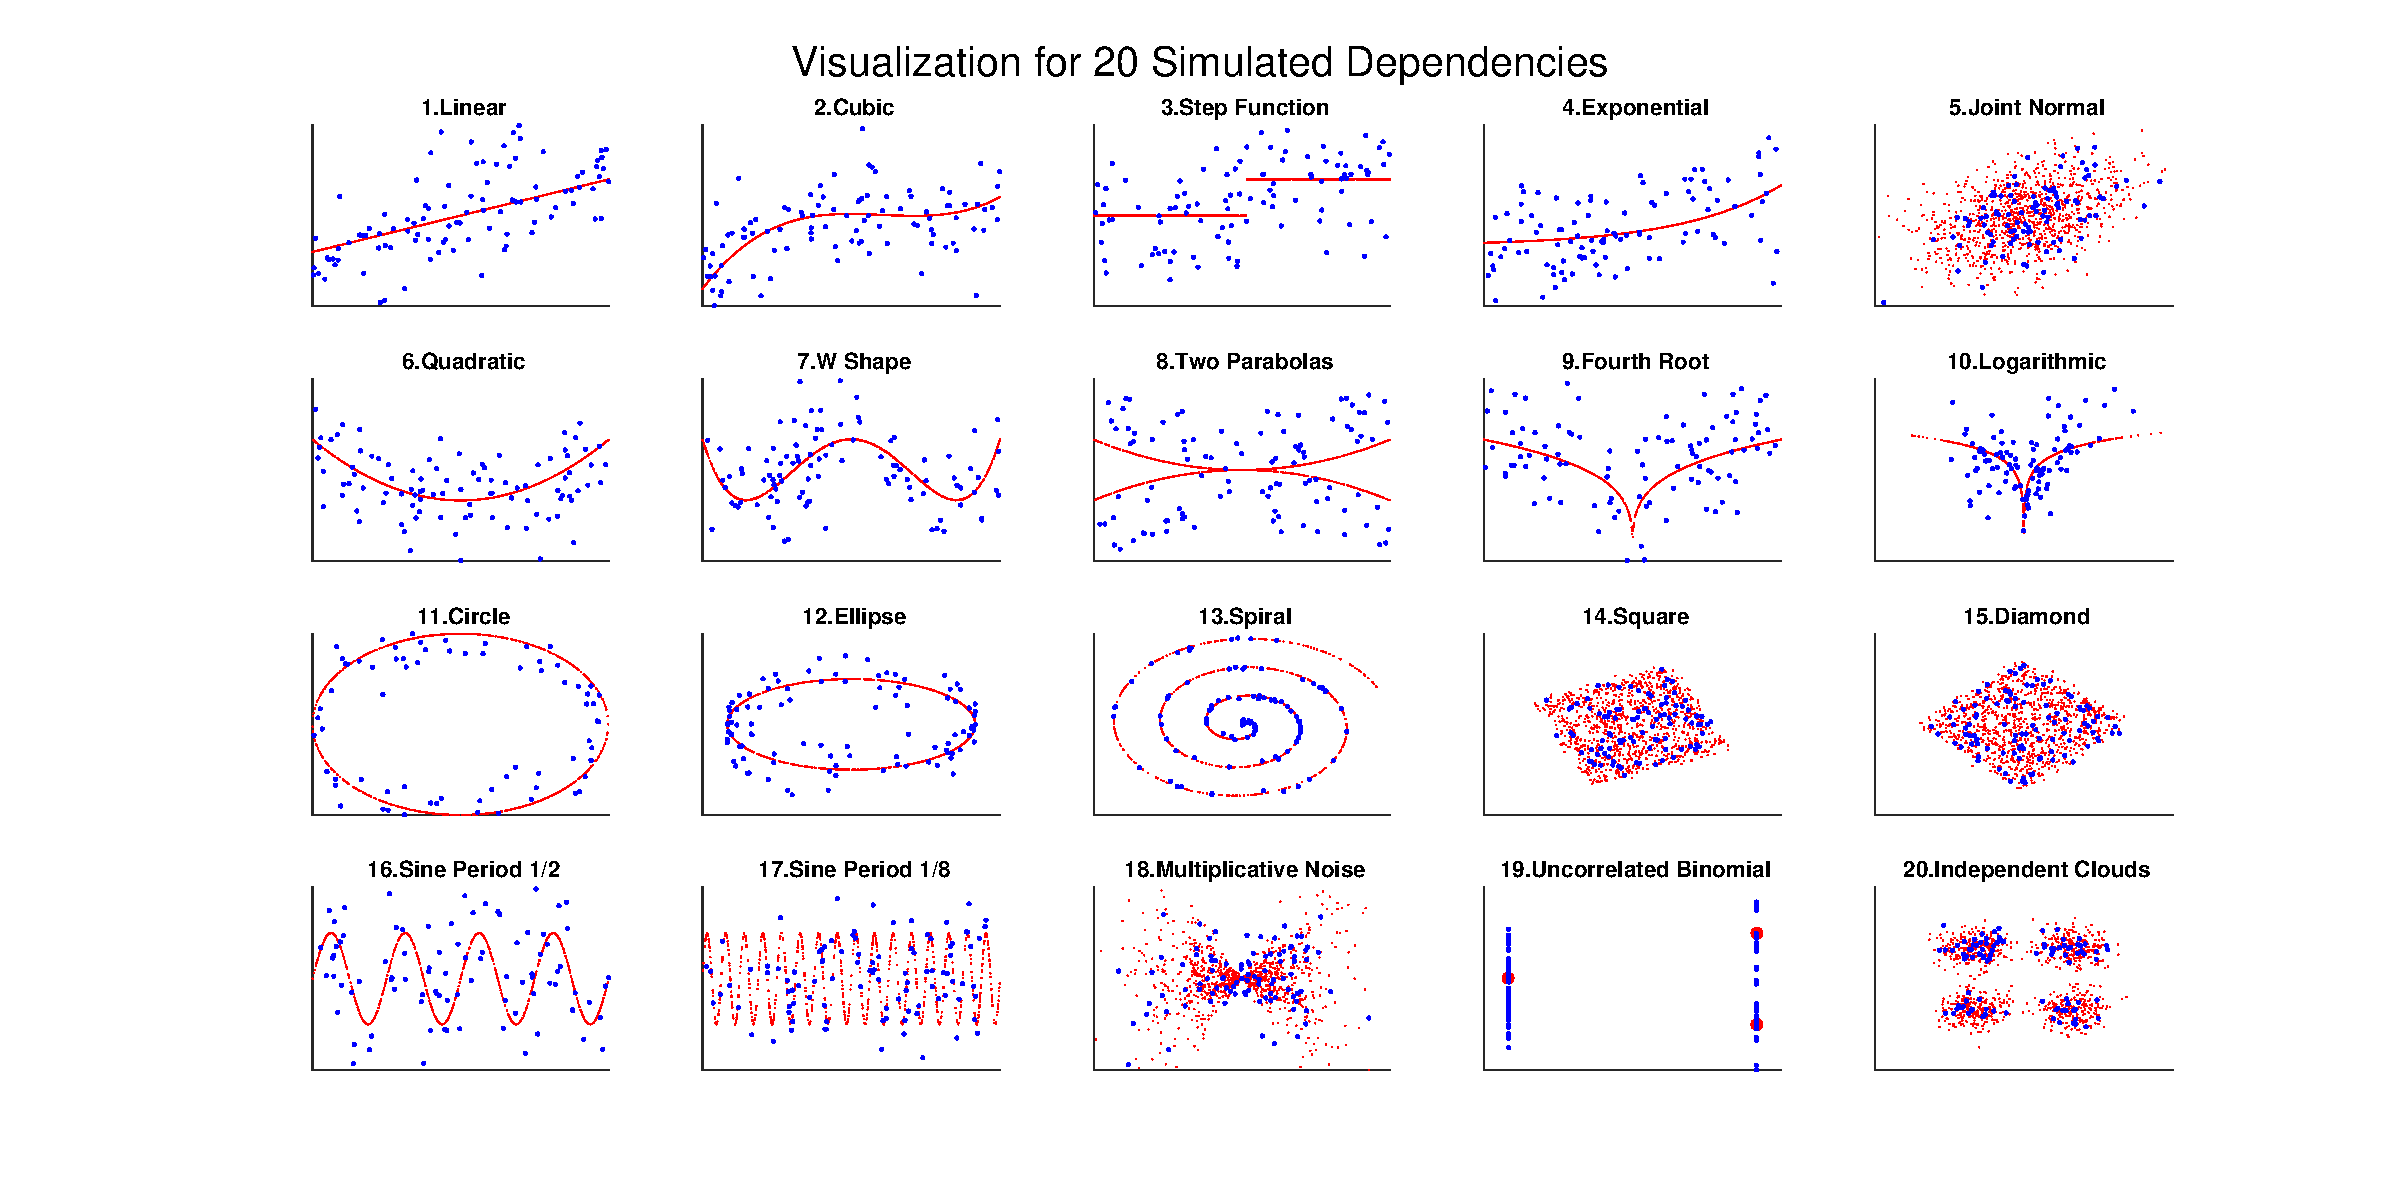
\includegraphics[trim={5cm 0 3.5cm 0},clip, width=1.0\textwidth]{../Figures/Fig0}
\caption{Visualization of 20 dependencies at dimension $1$. The blue points are generated with noise (c=1) for $n=100$ to show the actual sample data in testing, and the red points are generated with no noise for $n=1000$ to highlight each underlying dependency.
}
\label{fig0}
\end{figure}

For each distribution, $\mb{x}$ and $\mb{y}$ are clearly dependent (except type 20); and we can easily generate dependent sample data $X$ and $Y$ from the above distributions for testing purpose.

The low-dimensional simulation is based on $d_{x}=d_{y}=1$ and $c=1$, with a visualization of all dependencies given in Figure~\ref{fig0}. Note that the parameter before $c$ (e.g., there is a $80$ before $c$ in type 2) is a tuned noise parameter for some dependencies, such that the testing power neither increases too fast nor too slow for given distribution: in the absence of noise and at dimension $1$, certain dependency like linear is very easy to be detected so that the testing powers of all methods converge to $1$ at very small $n$, which causes difficulty in comparing the methods; it is also more meaningful to consider noisy scenarios in practice. 

The high-dimensional simulation is based on $c=0$ and increasing $d_{x}$, with $d_{y}=d_{x}$ for type $5,10,14,15,18,20$ and $d_{y}=1$ otherwise. For most dependencies, we use the decaying vector $w$ to treat later dimensions as small perturbation, such that the independence testing becomes more difficult as $d_{x}$ increases; but for some complex dependencies especially like square/diamond/sine period, the testing is already very difficult and $w$ is not used.

\section{Performance Profiles}
\label{appen:profiles}
The performance profiles are drawn by the following steps:

Suppose there are $S$ methods and $T$ different problems, and we denote the respective powers as $\beta_{\alpha}^{t}(s)$ for $s=1,\ldots,S$ and $t=1,\ldots,T$ at a fixed type 1 error $\alpha$. Then the relative performance for each method is defined as follows:
\begin{align*}
performance_{s}(x) &= \frac{1}{T} \sum_{t=1}^{T} \mb{I}((\beta_{\alpha}^{t}(*)-\beta_{\alpha}^{t}(s)) \leq x)
\end{align*}
where $x \in [0,1]$, $\mb{I}$ is the indicator function, and $\beta_{\alpha}^{t}(*) =\max_{s} \{\beta_{\alpha}^{t}(s)\}$ denotes the best testing power in the $t$th problem. Namely $x$ stands for the difference with respect to the best power, and the relative performance of each method equals the proportion of simulations that the method is worse than the best method by no more than $x$. For example, at $x=0.1$, MGC has a relative performance of $0.75$ if and only if there are $15$ out of $20$ simulations that MGC is worse than the best method by no more than $0.1$ in testing power. 

Note that the performance profiles at $x=0$ stands for the proportion of simulations that the method has the best power; and the curve always increases to $1$ at $x=1$. 

\section{Dependence Measures}
\label{appen:methods}

In this section, we review the Mantel test, distance correlation, modified distance correlation, and the HHG statistic in order. They all start with two Euclidean distance matrices $C=(c_{ij}), D=(d_{ij}) \in \Real^{n \times n}$, where $c_{ij}=\|x_{i}-x_{j}\|_{2}$ and $d_{ij}=\|y_{i}-y_{j}\|_{2}$. 

\subsection{(Global) Mantel Test}
\label{appen:mantel}
Given two Euclidean distance matrices $C$ and $D$ for $X$ and $Y$, the Mantel coefficient \cite{Mantel1967} is defined as 
\begin{equation}
Mantel(X,Y)=\frac{\sum_{i \neq j}^{n}(c_{ij}-\hat{E}(C))(D_{ij}-\hat{E}(D))}{\sqrt{\sum_{i \neq j}^{n}(c_{ij}-\hat{E}(C))^2 \sum_{i \neq j}^{n}(d_{ij}-\hat{E}(D))^2}},
\end{equation}
where $\hat{E}(C)=\frac{1}{n(n-1)}\sum_{i \neq j}^{n}(c_{ij})$ and similarly for $\hat{E}(D)$. In terms of the general correlation coefficient in Equation~\ref{generalCoef}, the Mantel coefficient essentially takes $a_{ij}=c_{ij}-\hat{E}(C)$ and $b_{ij}=d_{ij}-\hat{E}(D)$ when $i \neq j$, and $a_{jj}=b_{jj}=0$.

Therefore, the Mantel coefficient treats the two distance matrices as two observation vectors and calculates the Pearson's product-moment correlation coefficient between them. Then the Mantel test is carried out by the permutation test.

Unlike distance correlation and HHG, the Mantel test is not consistent against all dependent alternatives; but it has been a very popular method in biology and ecology due to its simplicity. Indeed we can observe from Figure~\ref{fig:nD} that the global Mantel coefficient is sub-optimal and appears to be not consistent for many dependencies; but multiscale graph correlation implemented by Mantel nevertheless achieves comparable performances as other variants of MGC, which implies that MGC$\{$Mantel$\}$ may be consistent against most, if not all dependent alternatives.

\subsection{(Global) Distance Correlation}
\label{appen:dcorr}
Given the Euclidean distance matrices $C$ and $D$, the sample distance covariance is defined on the doubly centered distance matrices $C^{H}$ and $D^{H}$:
\begin{equation}
\label{dcovEqu}
dcov(X,Y)=\frac{1}{n^2}\sum_{i,j=1}^{n}c^{H}_{ij}d^{H}_{ij},
\end{equation}
where $C^{H}=HCH$, $D^{H}=HDH$ with $H=I_{n}-\frac{J_{n}}{n}$. Then the sample distance variance is defined as
\begin{align*}
dvar(X) &=\frac{1}{n^2}\sum_{i,j=1}^{n}c^{H}_{ij}d^{H}_{ij}\\
dvar(Y) &=\frac{1}{n^2}\sum_{i,j=1}^{n}c^{H}_{ij}d^{H}_{ij},
\end{align*}
and the sample distance correlation follows as
\begin{equation}
\label{dcorrEqu}
dcorr(X,Y)=\frac{dcov(X)}{\sqrt{dvar(X) \cdot dvar(Y)}}.
\end{equation}
In the form of the general correlation coefficient in Equation~\ref{generalCoef}, distance correlation takes $a_{ij}=c^{H}_{ij}$ and $b_{ij}=d^{H}_{ij}$ for all $i,j$.

It is shown in \cite{SzekelyRizzoBakirov2007} that as $n \rightarrow \infty$, $dcorr(X,Y) \rightarrow dcorr(\mb{x},\mb{y}) \geq 0$, where $dcorr(\mb{x},\mb{y})$ denotes the population distance correlation between the random variables $\mb{x}$ and $\mb{y}$. The population distance correlation is defined by the characteristic functions, which is $0$ if and only if $\mb{x}$ and $\mb{y}$ are independent. Thus the sample distance correlation is a consistent test statistic for independence, i.e., the testing power $\beta_{\alpha}(dcorr(X,Y))$ converges to $1$ as $n$ increases, at any fixed type $1$ error level $\alpha$. 

Note that the consistency result assumes finite second moments of $\mb{x}$ and $\mb{y}$, and the consistency holds for a family of metrics including the Euclidean distance \cite{Lyons2013}. Furthermore, all of $dcov, dvar, dcorr$ are always non-negative; and the $dcorr$ defined here is actually the square of distance correlation in \cite{SzekelyRizzoBakirov2007}, but for simplicity we drop the square naming here.

\subsection{(Global) Modified Distance Correlation}
\label{appen:mcorr}
In case of high-dimensional data where the dimension $d_{x}$ or $d_{y}$ increases with the sample size $n$, the distance correlation $dcorr$ may no longer be appropriate. For example, even for independent Gaussian distributions, $dcorr(X,Y) \rightarrow 1$ as $d_{x}, d_{y} \rightarrow \infty$, which may severally impair the testing power of dcorr in high dimension simulations.

To tackle this problem, the modified distance correlation is proposed in \cite{SzekelyRizzo2013a}. The modified distance covariance is defined as
\begin{equation}
\label{mcovEqu}
mcov(X,Y)=\frac{n}{(n-1)^2(n-3)}(\sum_{i \neq j}^{n}c^{M}_{ij}d^{M}_{ij}-\frac{2}{n-2}\sum_{j=1}^{n}c^{M}_{jj}d^{M}_{jj}),
\end{equation}
where $C^{M}$ modifies the entries of $C^{H}$ by
\[c^{M}_{ij} = \left\{
  \begin{array}{lr}
    c^{H}_{ij}-\frac{c_{ij}}{n}, & \mbox{ if } i \neq j \\
    \frac{n\sum_{i}c_{ij}-\sum_{i,j}c_{ij}}{n^2}, &\mbox{ if } i = j 
  \end{array}
\right.
\]
and similarly for $D^{M}$. Then $mvar(X)$ can be defined by replacing all $d^{M}_{ij}$ in Equation~\eqref{mcovEqu} by $c^{M}_{ij}$, similarly for $mvar(Y)$. 

If $mvar(X) \cdot mvar(Y) \leq 0$, the modified distance correlation is set to $0$ (negativity can only occur when $n\leq 2$, equality can only happen in very special cases); otherwise it is defined as
\begin{equation}
\label{mcorrEqu}
mcorr(X,Y)=\frac{mcov(X,Y)}{\sqrt{mvar(X) \cdot mvar(Y)}}.
\end{equation}
In the form of the general correlation coefficient, modified distance correlation takes $a_{ij}=c^{M}_{ij}$ and $b_{ij}=d^{M}_{ij}$ for $i \neq j$, and $a_{jj}=\sqrt{-\frac{2}{n-2}}c^{M}_{jj}$ and $b_{jj}=\sqrt{-\frac{2}{n-2}}d^{M}_{jj}$. Note that since the diagonals are complex numbers, we will tweak them (without changing its theoretical consistency) when we implement multiscale graph correlation by mcorr, see in Section~\ref{appen:MGC}.

It is shown in \cite{SzekelyRizzo2013a} that $mcorr(X,Y)$ is an unbiased estimator of the population distance correlation $dcorr(\mb{x},\mb{y})$ for all $d_{x}, d_{y}, n$; and $mcorr$ is approximately normal even if $d_{x},d_{y} \rightarrow \infty$. Thus it is also a consistent test statistic for independence, but may work better than dcorr under high-dimension dependencies. 

%To summarize dcorr and mcorr, both methods are great for testing independence of Euclidean data due to their theoretical consistency, with the modified test statistic being more superior under high-dimensional dependency; and it is a flourishing concept by a series of papers \cite{BakirovRizzoSzekely2006, SzekelyRizzoBakirov2007, SzekelyRizzo2009, BickelXu2009, Kosorok2009, Remillard2009, LiZhongZhu2012, Lyons2013, SzekelyRizzo2013a, SzekelyRizzo2013b, SzekelyRizzo2014}. However, the required sample size for achieving a good testing power very much depends on the type of dependency underlying the given data, e.g. for perfect linear relationship, distance correlation usually requires less than $10$ points for a permutation test to declare significance; but for some nonlinear relationships like circle, distance correlation yields no significance even at $n=100$. Because real data rarely exhibits perfect linear relationship, and in practice large amount of data may not always be available, a better finite-sample method is of tremendous value: it not only yields a better testing power for the same sample size, but may also requires much less sample data for the permutation test to declare significance, which in turn saves the running time and data collection process. 

\subsection{Heller, Heller \& Gorfine (HHG)}
\label{appen:hhg}
Like dcorr and mcorr, the HHG statistic in \cite{HellerGorfine2013} is also distance-based and consistent; and like our multiscale graph correlation, it makes use of the rank information, but in a different manner. It applies Pearson's chi-square test to ranks of distances within each column, and is shown to be better than many global statistics including dcorr under many common nonlinear dependencies in \cite{GorfineHellerHeller2012, HellerGorfine2013}. 

Given the Euclidean distance matrices $C=[c_{ij}]$ and $D=[d_{ij}]$, we denote
\begin{align*}
H_{11}(i,j) &= \sum_{q=1,q\neq i,j}^{n}I(c_{ik} \leq c_{ij})I(d_{ik} \leq d_{ij}) \\
H_{12}(i,j) &= \sum_{q=1,q\neq i,j}^{n}I(c_{ik} \leq c_{ij})I(d_{ik} > d_{ij}) \\
H_{21}(i,j) &= \sum_{q=1,q\neq i,j}^{n}I(c_{ik} > c_{ij})I(d_{ik} \leq d_{ij}) \\
H_{22}(i,j) &= \sum_{q=1,q\neq i,j}^{n}I(c_{ik} > c_{ij})I(d_{ik} > d_{ij}).
\end{align*}
Then the HHG test statistic is
\begin{align*}
HHG(X,Y) &= \sum_{i=1,j\neq i}^{n} \frac{(n-2)(H_{12}(i,j)H_{21}(i,j)-H_{11}(i,j)H_{22}(i,j))^2}{H_{1 \cdot}(i,j)H_{2 \cdot}(i,j)-H_{\cdot 1}(i,j)H_{\cdot 2}(i,j)},
\end{align*}
where $H_{1 \cdot}=H_{11}+H_{12}$, $H_{2 \cdot}=H_{21}+H_{22}$, $H_{\cdot 1}=H_{11}+H_{21}$, and $H_{\cdot 2}=H_{12}+H_{22}$. The permutation test using the HHG statistic is consistent against all dependent alternatives.

It is clear that the HHG statistic is structurally different from Mantel/dcorr/mcorr, and cannot be expressed in terms of the general correlation coefficient in Equation~\ref{generalCoef}. Thus multiscale graph correlation cannot be directly implemented by HHG.

In our numerical simulations, HHG falls a bit short when testing against high-dimensional or close to linear dependencies, and it is quite sensitive to noises and perturbations. But it is much more advantageous than other global statistics under most nonlinear dependencies, which makes it a strong competitor. %However, Multiscale Graph Correlation is able to approximate or surpass its performances in most cases.

\section{Multiscale Graph Correlation}
\label{appen:MGC}

For any test statistic that can be expressed by the general correlation coefficient in Equation~\ref{generalCoef}, its multiscale graph correlation can be implemented by Equation~\ref{localCoef}. As an example, here we show how multiscale graph correlation is implemented by modified distance correlation, as well as explaining some implementation issues.

By section~\ref{appen:mcorr}, modified distance correlation is equivalent to the general correlation coefficient by taking $a_{ij}=c^{M}_{ij}$ and $b_{ij}=d^{M}_{ij}$ for $i \neq j$, and $a_{jj}=\sqrt{-\frac{2}{n-2}}c^{M}_{jj}$ and $b_{jj}=\sqrt{-\frac{2}{n-2}}d^{M}_{jj}$. But if we implement multiscale graph correlation by mcorr directly based on Equation~\ref{localCoef}, $g_{kl}$ may be a complex number when ties occur, e.g., $rank(a_{ij})=0$ and $rank(b_{ij})>0$.

Note that $a_{jj}$ and $b_{jj}$ converge to $0$, and the expectations of $c^{M}_{jj}$ and $d^{M}_{jj}$ are also $0$. Therefore, instead of using complex number diagonals, we can let $a_{jj}=b_{jj}=0$ with little inferential impact. Then the local variants of modified distance covariance becomes
\begin{align*}
mcov_{kl}(X,Y) = \frac{n}{(n-1)^2(n-3)}(\sum_{i \neq j}^{n}c^{M}_{ij}d^{M}_{ij}I(0<rank(a_{ij})<k))I(0<rank(b_{ij})<l),
\end{align*}
similarly for $mvar_{k}$, and eventually $mcorr_{kl}$ as the local test statistic of mcorr. After the above tweak to the diagonals, MGC$\{$mcorr$\}$ maintains its consistency, has little performance difference from before, and is still superior under high-dimensional dependencies.

There exists another problem for ties, which is of particular importance for MGC$\{$mcorr$\}$: modified distance correlation improves over the original distance correlation, mostly because its adjustment to the diagonal terms; and if there are repeating points in the data, it is necessary to adjust them in the same manner as the diagonal terms, or mcorr will lose its advantage and not function properly in a permutation test. Although repeating data happen with probability $0$ for data generated by continuous distributions, it can happen for discrete distribution and during resampling.

The tie problem is handled by taking minimal rank among ties, and let $a_{ij}$ equal $a_{jj}$ whenever $x_{i}=x_{j}$ (or any $x_{i}$ that is rank zero) in Equation~\ref{localCoef2}. This is necessary for any global correlation coefficient that $a_{jj}$ can be different from $a_{ij}$ when $x_{i}=x_{j}$, such as Mantel or mcorr; but does not matter for dcorr, for which $a_{jj}=a_{ij}$ always holds when $x_{i}=x_{j}$. As long as $a_{ij}$ is handled properly when $x_{i}=x_{j}$, in practice one can break the ties randomly or use min/average/max ranks without affecting the power of MGC.

Last but not least, in the local family of statistics it suffices to exclude $g_{1l}$ and $g_{k1}$: since $g_{1l}=g_{k1}=g_{11}$, they do not consider any neighbor, merely count the diagonal terms in the distance matrices, and are not meaningful for testing purpose. Therefore they are not considered in our main algorithm.

\section{Testing Procedure}
\label{appen:tests}

In this section we elaborate on the testing procedure by multiscale graph correlation used in the simulation and the real data experiment. 

In subsection~\ref{appen:algorithms} we present three essential algorithms for testing: given the global correlation coefficient, the first algorithm computes all local correlations between two sample data sets; the second algorithm computes the testing powers of the local correlations, based on given joint distribution or given observations; and the third algorithm computes the p-value of the local statistics by a random permutation test. 

In subsection~\ref{appen:eval}, we show how the three core algorithms are combined, to yield the testing powers of MGC in the simulations and the p-values of MGC in the real data experiment.

\subsection{Algorithms}
\label{appen:algorithms}
The three algorithms are implemented in Matlab and R, with the pseudo-code shown in Algorithm~\ref{algLGC},~\ref{algPower},~\ref{algPerm}.

The first algorithm is the core to evaluate MGC in all other algorithms, which computes all local correlations based on given distance matrices $C$ and $D$. The function calculates Equation~\ref{localCoef} for all scales, which is clear in concept; but some matrix manipulations are required to efficiently implement it. Note that a priori assumption is a global function that returns $\{a_{ij}\},\{b_{ij}\}$ and the ranks, according to the choice of the global coefficient coefficient.

The second algorithm computes the testing powers of all local statistics, by either repeated simulating samples generated by the joint distribution $f_{xy}$, or bootstrap samples of the given observations $(X, Y)$ with smoothing. This algorithm is required for MGC to estimate the optimal scale among all neighborhoods by maximizing the powers among all local statistics; and we explain and validate the smoothing technique in Section~\ref{appen:justi}.

The third algorithm computes the p-values of all local statistics by the permutation test. This algorithm is straightforward to implement, and is used to output the p-values of all local tests for given real data.

The complexity of Algorithm~\ref{algLGC} is $O(n^2 \log n)$: the global function takes $O(n^2 \log n)$, and the following loops take $O(n^2)$. Algorithm~\ref{algPower} takes $O(rn^2 \log n)$: it takes $O(rn^2 \log n)$ to generate data and calculate the test statistics, and $O(n^2 (r+\log n))$ to estimate the power. Algorithm~\ref{algPerm} takes $O(rn^2 \log n)$ as well. 

Note that all three algorithms can be used for global mcorr/dcorr/Mantel/HHG, by excluding the respective local parts, i.e., in Algorithm~\ref{algLGC}, the loops after the global function are not needed for global correlation; in Algorithm~\ref{algPower} and Algorithm~\ref{algPerm}, the powers and p-values only need to be estimated for one global correlation rather than $n^2$ local statistics. Therefore, for HHG (in general, any global correlation involving sorting, or the local test at the optimal scale), the complexity of each algorithm is the same as before but slightly less in actual running time; and for global mcorr/dcorr/Mantel, the complexity of each algorithm becomes $O(n^2), O(rn^2), O(rn^2)$ since sorting is no longer needed.

\begin{algorithm}
\caption{Local Correlations}
\label{algLGC}
\begin{algorithmic}
\Function{LGC}{$C$,$D$,option}  \Comment{option specifies the global correlation in use}
\State initialize an $n \times n$ matrix $corrXY$, and two vectors $varX$ and $varY$ of size $n \times 1$;
\State $[a,b,rkA,rkB]=global(C,D,option)$; \Comment{all outputs are size $n \times n$}
\For{$j=1,\ldots,n$}
\For{$i=1,\ldots,n$}
\State $ra=rkA$; $rb=rkB$;
\If{$ra==0$}
\State $a_{ij}=a_{jj}$; \Comment{adjust entries corresponding to repeating points}
\EndIf
\If{$rb==0$}
\State $b_{ij}=b_{jj}$;
\EndIf
\State $ra=ra+1$; $rb=rb+1$;
\State $corrXY(ra, rb)=corrXY(ra, rb)+a_{ij}b_{ij}$;
\State $varX(ra)=varX(ra)+a_{ij}^2$;
\State $varY(rb)=varY(rb)+b_{ij}^2$;
\EndFor
\EndFor

\For{$j=1,\ldots,n-1$}
\State $corrXY(1, j+1)=corrXY(1, j)+corrXY(1, j+1)$;
\State $corrXY(j+1,1)=corrXY(j+1,1)+corrXY(j+1,1)$;
\State $varX(j+1)=varX(j)+varX(j+1)$;
\State $varY(j+1)=varY(j)+varY(j+1)$;
\EndFor

\For{$j=1,\ldots,n-1$}
\For{$i=1,\ldots,n-1$}
\State $corrXY(i+1,j+1)=corrXY(i+1,j)+corrXY(i,j+1)+corrXY(i+1,j+1)-corrXY(i,j)$;
\EndFor
\EndFor
\State $corrXY=corrXY./\sqrt{(varX) (varY)^{T}}$; \Comment{$./$ means entry-wise division}
\State \Return $corrXY$;
\Comment{the local test statistics $g_{kl}=corrXY(k,l)$ for each $k,l=1,\ldots,n$}
\EndFunction
\end{algorithmic}
\end{algorithm}

\begin{algorithm}
\caption{Testing Power Estimation}
\label{algPower}
\begin{algorithmic}
\Function{TestingPowers}{$X$,$Y$,$f_{xy}$,$r$,$\alpha$,option} 
\State initialize two $n \times n \times r$ array $testN$ and $testA$ to store the local test statistics under the null and the alternative, and an $n \times n$ matrix $power$ to store the empirical power of all local tests at type 1 error level $\alpha$;
\For{$m=1,\ldots,r$} 
\If{$f_{xy}$ is given}
\State $(X_{1},Y_{1})=generateData(f_{xy})$; \Comment{generate dependent $(X_{1},Y_{1})$}
\State $(X_{2},Y_{2})=generateData(f_{xy})$; \Comment{generate an independent $Y_{2}$}
\State $C_{1}=dist(X_{1})$; $D_{1}=dist(Y_{1})$; $D_{2}=dist(Y_{2})$;\Comment{calculate the distance matrices}
\Else
\State $perA=randsampling(n)$;
\State $C_{1}=dist(X(:,perA))$; $D_{1}=dist(Y(:,perA))$; \Comment{dependent distance matrices}
\State $perN=randsampling(n)$;
\State $D_{2}=dist(Y(:,perN))$; \Comment{re-sample the second data}
\State $Z=generateData('normal')$;\Comment{generate a matrix of size $n \times 1$ by standard normal distribution}
\State $E_{1}=dist(Z)$;
\EndIf
\State $testA(:,:,m)=LGC(C_{1},D_{1},option)+LGC(E_{1},D_{1},option)*100$; 
\State $testN(:,:,m)=LGC(C_{1},D_{2},option)+LGC(E_{1},D_{2},option)*100$;
\EndFor

\For{$j=1,\ldots,n$}
\For{$i=1,\ldots,n$}
\State $testN(i,j,:)=sort(testN(i,j,:),'decreasing')$; 
\State $cut=testN(i,j,ceil(r\alpha))$; \Comment{estimate the critical value at level $\alpha$}
\State $power(i,j)=mean(testA(i,j,:)>cut)$; \Comment{estimate the power}
\EndFor
\EndFor
\State \Return $power$.
\EndFunction
\end{algorithmic}
\end{algorithm}

\begin{algorithm}
\caption{P-value Estimation}
\label{algPerm}
\begin{algorithmic}
\Function{PermutationTest}{$X$,$Y$,$r$,option}
\State initialize an $n \times n$ matrix $p$ to store the p-values of all local tests;
\State $C=dist(X)$; $D=dist(Y)$; \Comment{calculate the distance matrices}
\State $cut=LGC(C,D,option)$; \Comment{calculate the observed test statistics}
\For{$m=1,\ldots,r$}
\State $per=randperm(n)$; \Comment{generate a random permutation}
\State $cut2=LGC(C,D(per,per),option)$; \Comment{calculate the permuted test statistics}
\For{$j=1,\ldots,n$}
\For{$i=1,\ldots,n$}
\If{$cut2(i,j)<cut(i,j)$}
\State $p(i,j)=p(i,j)+1/r$;
\EndIf
\EndFor
\EndFor
\EndFor
\State \Return $p$.
\EndFunction
\end{algorithmic}
\end{algorithm}

\subsection{Evaluation of MGC}
\label{appen:eval}

To evaluate MGC in simulations or real data, we first need to estimate the optimal scale of MGC. By running Algorithm~\ref{algPower}, it estimates the testing powers $\hat{\beta}_{\alpha}(g_{kl})$ of all local statistics, so the optimal scale can be estimated by maximizing the empirical powers:
\begin{equation}
\label{power}
(k^{*},l^{*})=\arg\max_{k,l \in [2,\ldots,n] }\{\hat{\beta}_{\alpha}(g_{kl})\}.
\end{equation}
If there are more than one optimal neighborhood choices, we take one optimal scale that maximizes $k^{*}l^{*}$; alternatively we can use all optimal scales and output the mean power/p-value. 

Once the optimal scale is estimated, the p-value of MGC can be calculated by running Algorithm~\ref{algPerm} at the optimal scale $(k^{*},l^{*})$. The testing power of MGC can be quickly determined by running Algorithm~\ref{algPower} again to estimate the power at the optimal scale $(k^{*},l^{*})$. 

We can apply the same procedures to evaluate the p-values and powers for global correlations like dcorr/mcorr/Mantel/HHG, by excluding the first step for estimating the optimal scale.

\subsection{Justification of MGC on using Noisy Samples}
\label{appen:justi}
In Algorithm~\ref{algPower}, when we estimate the optimal scale of MGC for given data of unknown distribution, we repeatedly add independent white noise to the given observations, and use the noisy samples to derive the testing power: for given distance matrix pair $(C,D)$, the testing power is derived by comparing $g_{kl}(C+E,D)$ to $g_{kl}(C+E,D')$, where $E$ is a distance matrix of $z$ that is independently generated by the normal distribution, and $D'$ is a random sample of $D$. 

But the question is whether the optimal scale based on the noisy samples is equivalent to the true optimal scale based on the underlying joint distribution. The next theorem shows that the optimal scale is invariant to the noise, which justified algorithm~\ref{algPower}.

\begin{thm}
\label{thm4}
Suppose $f_{xy}$ is the true underlying distribution of the given data $(X,Y)$.

Then in algorithm~\ref{algPower}, the testing power estimated by the noisy samples can be arbitrarily close to the testing power based on the underlying distribution as the number of replicates increases.

Thus the optimal scale estimated by the noisy samples approximates the true optimal scale.
\end{thm}

Rather than using large noise (the noise in algorithm~\ref{algPower} is set to have the same Frobenius norm as the signal), it is tempting to estimate the optimal scale by smaller noise level, or more simply by resampling the given data without noise. Both choices are still valid under Theorem~\ref{thm4} for estimating the optimal scale, but may introduce additional bias in the following step in estimating the MGC p-value or testing power: if the optimal scale is estimated by resamples of given data, the optimal scale is dependent on the data while the follow-on permutation test is also dependent on the given data, such that the resulting p-value can be biased, e.g., the MGC p-value can be too low and the MGC testing power can be higher than the type $1$ error level under independence.

In comparison, when the optimal scale is estimated based on repeated simulating samples of $f_{xy}$, the optimal scale is estimated independently of the MGC p-value or testing power in the following step. This is the most ideal way to estimate the optimal scale, which does not introduce any bias; but it is in general difficult to fit a model for given observations.

By Theorem~\ref{thm4}, no matter how large the noise level, the optimal scale can always be reasonably estimated, while small or no noise level may introduce additional bias into the p-value and testing power. Therefore in algorithm~\ref{algPower} the noise level is set to be the same as the signal, in order to diminish the dependency between the optimal scale estimation and the permutation test on the given data. For example, in the real data experiment on testing non-existent stimulus, the MGC testing power is very close to the type $1$ error level $0.05$; but if we reduce the noise level or simply use bootstrap resamples, the MGC testing power will be inflated to around $0.1$. 

\section{Proofs}
\label{appen:proofs}
%Although distance correlation is already consistent against all alternatives, it may not always yield a good finite-sample testing power for a particular dependency type; while our Multiscale Graph Correlation is able to improve the testing power by choosing the best neighborhood for a given joint distribution. 

%The advantage of using k-nearest-neighbor in distance matrices, lies in its capability to exclude the product of small distances in one data set and large distances in the other data set: after double centering, the centered small distance is usually negative and the centered large distance is usually positive, and including such product reduces the magnitude of local distance covariance under the alternative. While excluding such product by k-nearest-neighbor can increase the magnitude of local distance covariance under the alternative, albeit at the cost of increasing its magnitude under the null as well. 

\begin{thm}
Suppose for given $f_{xy}$ and $\alpha$, $\beta_{\alpha}(g_{nn}) \rightarrow 1$ as $n \rightarrow \infty$ for given $f_{xy}$ and $\alpha$, then $\beta_{\alpha}(g) \rightarrow 1$ as well.

Therefore, multiscale graph correlation is consistent against all dependent alternatives of finite second moments, when it is implemented by distance correlation or modified distance correlation.
\end{thm}
\begin{proof}
The power of multiscale graph correlation satisfies
\begin{equation}
\beta_{\alpha}(g)=\max_{k,l \in [2,\ldots,n]}\{\beta_{\alpha}(g_{kl})\} \geq \beta_{\alpha}(g_{nn}).
\end{equation}
So if $\beta_{\alpha}(g_{nn}) \rightarrow 1$, we also have $\beta_{\alpha}(g) \rightarrow 1$.

Since dcorr and mcorr are consistent against all alternatives of finite second moments by \cite{SzekelyRizzoBakirov2007, SzekelyRizzo2013a}, clearly their multiscale graph correlations are also consistent.
\end{proof}

\begin{thm}
Suppose $\mb{y}=c\mb{x}$ for a non-zero scalar $c$. Then for any $n$ and $\alpha$ it always holds that
\begin{equation}
\beta_{\alpha}(g) = \beta_{\alpha}(g_{nn}).
\end{equation}

Thus multiscale graph correlation is equivalent to the global correlation coefficient under linear dependency.
\end{thm}
\begin{proof}
To show that MGC is no better than its global correlation coefficient, it suffices to show the p-value of $g_{kl}$ is always no less than the p-value of $g_{nn}$ for all $k,l$.

%Let us first suppose $\mb{x}$ is continuously distributed, such that with probability $1$ no two columns of $X$ have the same magnitude.

Under linear dependency, for any global correlation coefficient satisfying Equation~\ref{generalCoef}, by Cauchy-Schwarz inequality we have
\begin{equation}
1=g_{nn}(X, Y) \geq g_{nn}(X, YQ)
\end{equation}
for any permutation matrix $Q$, for which the equality holds if and only if $X$ is a scalar multiple of $YQ$. It follows that the p-value of $g_{nn}$ is $\frac{|\Omega|}{n!}$, where $|\Omega|$ equals the cardinality of $\Omega=\{Q, X \mbox{ is a scalar multiple of }YQ\} \subset \{\mbox{all possible permutation matrices }Q\}$. Since the identity matrix is an element of $\Omega$, the p-value of $g_{nn}$ is at least $\frac{1}{n!}$.

For any $Q \in \Omega$ and any $k,l$, clearly $g_{kl}(X,Y)=g_{kl}(X,YQ)$. It follows that the p-value of $g_{kl}$ is no less than $\frac{|\Omega|}{n!}$; and there may exist other permutation matrices $Q \notin \Omega$ such that $g_{kl}(X,Y) \leq g_{kl}(X,YQ)$. Thus the p-value of $g_{kl}$ is always bounded below by the p-value of $g_{nn}$.

Therefore for any $k,l$, we must have $\beta_{\alpha}(g_{kl}) \leq \beta_{\alpha}(g_{nn})$. Since multiscale graph correlation includes the global test statistic and equals the optimal test statistic in the family, it follows that $\beta_{\alpha}(g) = \beta_{\alpha}(g_{nn})$ at any given type $1$ error level $\alpha$.

Note that this theorem holds for MGC based on any of mcorr/dcorr/Mantel.
\end{proof}

\begin{thm}
There exists $f_{xy}$, $n$ and $\alpha$ such that 
\begin{equation}
\beta_{\alpha}(g) > \beta_{\alpha}(g_{nn}).
\end{equation}

Thus multiscale graph correlation can be better than its global correlation coefficient under certain nonlinear dependency.
\end{thm}
\begin{proof}
We give a simple discrete example of $f_{xy}$ at $n=7$, such that the p-value of $g_{kl}$ for some $(k,l) \neq (n,n)$ is strictly lower than the p-value of $g_{nn}$. This is equivalent to say the permutation test power $\beta_{\alpha}(g)$ is larger than $\beta_{\alpha}(g_{nn})$ at an appropriate type $1$ error level $\alpha$.

Suppose under the alternative, $f_{xy}$ is distributed as follows:
\begin{align*} 
\mb{x} &\in \{-1,-\frac{2}{3},-\frac{1}{3},0,\frac{1}{3},\frac{2}{3},1\} \mbox{ without replacement}, \\
\mb{y} &= \mb{x}^2,
\end{align*}
which is a discrete version of the quadratic relationship in the simulations.

In this example we can easily consider all possibilities of $C^{M}$ and $D^{M}$, and calculate $g_{kl}(X, Y)$ and $\{g_{kl}(X, YQ)\}$ for all permutation matrices $Q$. Take $g_{nn}=mcorr, n=l=7, k=2$ as an example, $g_{nn}(X, Y)=0.0783$, $g_{kl}(X, Y)=0.0583$, and similarly all possible permuted test statistics. It follows that the p-value of $g_{nn}$ is $0.2683$, while the p-value of $g_{kl}$ is $0.1571$. 

Therefore we have an example of $f_{xy}$ and $n$ such that $\beta_{\alpha}(g_{kl}) > \beta_{\alpha}(g_{nn})$ for some $(k,l) \neq (n,n)$: by choosing $\alpha=0.2, n=7$, we have $1=\beta_{\alpha}(g_{kl}) > \beta_{\alpha}(g_{nn})=0$ at $(k,l)=(2,7)$. Then $\beta_{\alpha}(g)=\max_{k,l}{\beta_{\alpha}(g_{kl})}=1>\beta_{\alpha}(g_{nn})$, and MGC$\{$mcorr$\}$ is better than the global mcorr.

Note that we can always consider equally spaced sample points (or randomly sampled points) in $[-1,1]$ for $X$, increase $n$ and reach the same conclusion with smaller p-values; but the computation of all possible permuted test statistics becomes much more time-consuming as $n$ increases. Furthermore, the same conclusion holds for MGC based on dcorr or Mantel using the same example.
\end{proof}

\begin{thm}
Suppose $f_{xy}$ is the true underlying distribution of the given data $(X,Y)$.

Then in algorithm~\ref{algPower}, the testing power estimated by the noisy samples can be arbitrarily close to the testing power based on the underlying distribution as the number of replicates increases.

Thus the optimal scale estimated by the noisy samples approximates the true optimal scale.
\end{thm}
\begin{proof}
For given known joint distribution $f_{xy}$, the testing power of $g_{kl}$ is based on the distance matrices $(C,D)$ of the repeated simulating samples $(X,Y)$ generated by $f_{xy}$. 

Take distance correlation for example, 

\begin{align*}
\label{localCoef}
g_{kl}^{'} &= \sum_{i,j=1}^n (a_{ij}+e_{ij}) b_{ij} I_{rank(a_{ij}+\epsilon_{a})<k} I_{rank(b_{ij}+\epsilon_{b})<l}  \\
& \rightarrow \sum_{i,j=1}^n (a_{ij}+e_{ij}) b_{ij} I_{rank(a_{ij})<k} I_{rank(b_{ij})<l}  \\
& = \sum_{i,j=1}^n a_{ij}b_{ij} I_{rank(a_{ij})<k} I_{rank(b_{ij})<l}  + \sum_{i,j=1}^n e_{ij}b_{ij} I_{rank(a_{ij})<k} I_{rank(b_{ij})<l}  \\
& = g_{kl} + g_{kl}^{''}
\end{align*}
since $E$ is independent of $A$ and $B$, $g_{kl}^{''}$


\begin{equation}
\label{dcovEqu}
dcov(X,Y)=\frac{1}{n^2}\sum_{i,j=1}^{n}c^{H}_{ij}d^{H}_{ij},
\end{equation}
where $C^{H}=HCH$, $D^{H}=HDH$ with $H=I_{n}-\frac{J_{n}}{n}$. Then the sample distance variance is defined as


\begin{equation}
\label{localCoef}
g_{kl}=\frac{\sum_{i,j=1}^n a_{ij}^k b_{ij}^l}{\sqrt{\sum_{i,j=1}^n  a_{ij}^{k} a_{ij}^{k} \sum_{i,j=1}^n b_{ij}^{l} b_{ij}^{l}}},
\end{equation}


In algorithm~\ref{algPower}, the testing power of $g_{kl}$ is based on the distance matrices $(C,D)$ generated by repeated simulating samples $(X,Y)$ of the known joint distribution $f_{xy}$


\end{proof}


\bibliographystyle{alpha}
\bibliography{references}

\end{document}